\documentclass[aps,pra,superscriptaddress,twocolumn]{revtex4-1}

\usepackage{graphicx}
\usepackage{amsmath}
\usepackage{amssymb}
\usepackage{hyperref}
\usepackage[utf8]{inputenc}
\usepackage{mathtools}
\usepackage[english]{babel}
\usepackage{bbm}
\hypersetup{colorlinks=true, linkcolor=blue, citecolor=blue, urlcolor=blue}
\usepackage{xcolor}
\usepackage{braket}

%===Newcommands============================
\DeclareMathOperator{\sgn}{sgn}
\newcommand{\ie}{i.\,e.,\ }
\newcommand{\Ie}{I.\,e.\,,\ }
\newcommand{\eg}{e.\,g.,\ }
\newcommand{\Eg}{E.\,g.\,,\ }
\newcommand{\cf}{cf.\ }
%
\newcommand{\re}{\mathrm{Re}}
\newcommand{\im}{\mathrm{Im}}
\newcommand{\abs}[1]{|#1|}
\newcommand{\ii}{\mathrm{i}}
\newcommand{\ee}{\mathrm{e}}
\newcommand{\proj}[1]{|#1\rangle\langle #1|}
\newcommand{\Tr}{\operatorname{Tr}}
\newcommand{\rr}{\mathbf{r}}
\newcommand{\pp}{\mathbf{p}}
\newcommand{\kk}{\mathbf{k}}
%
\newcommand{\cc}{\text{c.c.}}
\newcommand{\fref}[1]{\text{Fig.}~\ref{#1}}
\newcommand{\ffref}[1]{\text{Figs.}~\ref{#1}}
\newcommand{\eref}[1]{\text{Eq.}~\eqref{#1}}
\newcommand{\eeref}[1]{\text{Eqs.}~\eqref{#1}}
%
\newcommand{\commentSB}[1]{\texttt{\color{blue}[#1]}}
\newcommand{\commentSO}[1]{\texttt{\color{orange}[#1]}}
\newcommand{\commentTP}[1]{\texttt{\color{green}[#1]}}
\newcommand{\commentOR}[1]{\texttt{\color{yellow}[#1]}}
\newcommand{\commentSY}[1]{\texttt{\color{red}[#1]}}

%==============================================================================================
\begin{document}
\title{Optimized geometries for optical lattices}
\author{A}
% \email{}
\affiliation{Department of Physics, Harvard University, Cambridge, Massachusetts 02138, USA}
\author{B}
% \email{}
\affiliation{Department of Physics, Harvard University, Cambridge, Massachusetts 02138, USA}
\author{C}
% \email{}
\affiliation{Department of Physics, Harvard University, Cambridge, Massachusetts 02138, USA}

\begin{abstract}

This is the abstract. 

\end{abstract}

\maketitle

%==============================================================================================
\section{Introduction}

% This is the introduction, see~\fref{fig:setup}.
% % \commentSB{not sure about this statement}

% \begin{equation}
% H = p^2
% \label{eqn:Hamiltonian}
% \end{equation}

\begin{figure}
\centering
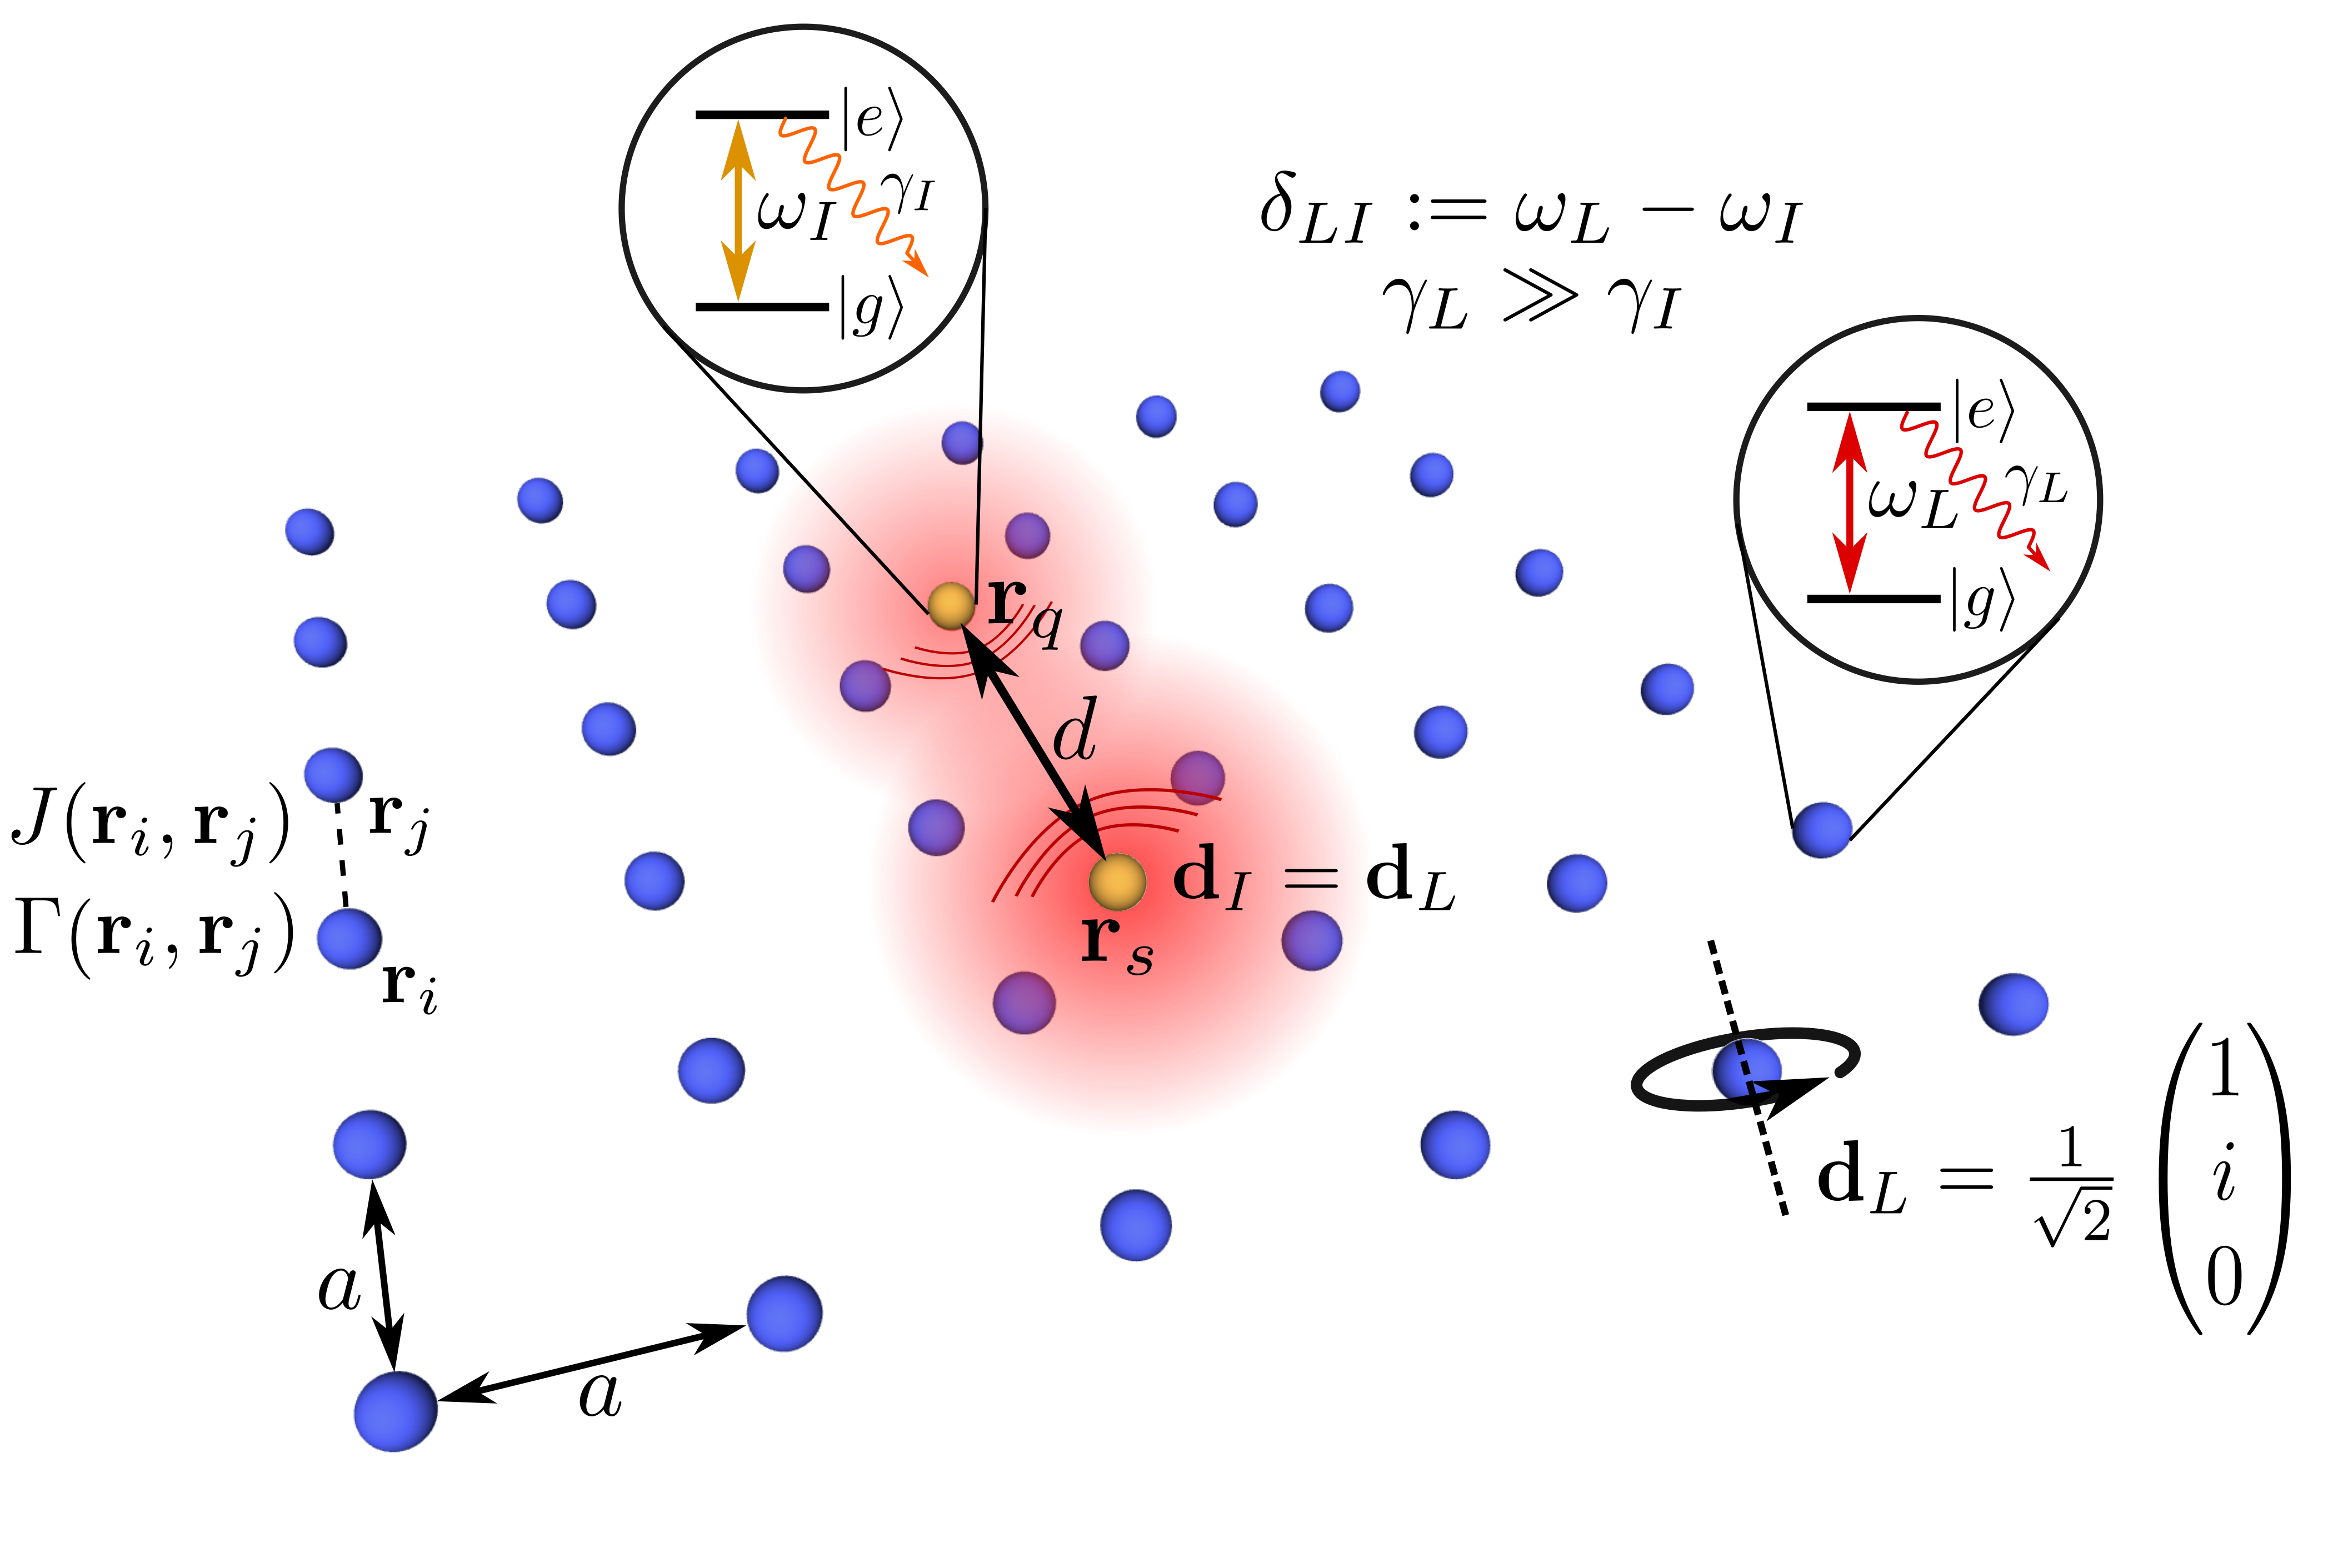
\includegraphics[width=0.4\textwidth]{figures/setup_2.png} 
\caption{•}
\label{fig:setup}
\end{figure}

% We see in~\eeref{eqn:Hamiltonian} and~\fref{fig:setup},~\eg test~\cite{kramer_quantumopticsjl_2018}

%==============================================================================================
\section{Model}
\commentSO{arb. geometry, Green's Tensor, Couplings, Polarizations -> Distance dependence, Hamiltonian, Self-energy, Ref. to Taylor's work}

We consider two-dimensional sub-wavelength lattices of quantum emitters which interact via resonant dipole-dipole interactions. The emitters are assumed to be two-level stems with a ground state $\ket{g}$ and an excited state $\ket{e}$ with a trasition frequency $\omega_L = c k_L$, such that $k_L = 2\pi/\lambda_L$ denotes the related wavenumber with the resonance wavelegth $\lambda_L$. Pairwise resonant dipole-dipole interactions among emitters result in collective couplings $J_{ij}$ and collective decay rates $\Gamma_{ij}$ between emitters $i$ and $j$ at positions $\rr_i$ and $\rr_j$, given by 
\begin{subequations}
    \begin{align} J_{ij} = -\frac{3\pi \sqrt{\gamma_i \gamma_j}}{\omega_L} {\hat{d}^\dagger}_i \cdot \textbf{Re} [\textbf{G}(\textbf{r}_{ij}, \omega_L)] \cdot \hat{d}_j 
    \label{eqn:J} \\
    \Gamma_{ij} = \frac{6\pi \sqrt{\gamma_i \gamma_j}}{\omega_L} {\hat{d}^\dagger}_i \cdot \textbf{Im} [\textbf{G}(\textbf{r}_{ij},\omega_L)] \cdot \hat{d}_j 
    \label{eqn:Gamma} 
    \end{align}
\end{subequations}

% \commentTP{Make this and all the others into subequations}
where $\gamma_i$ and $\gamma_j$ are the decay rates of the individual dipoles $i$ and $j$, and $\rr_{ij} = \rr_i - r_j$ is the displacement vector. $\textbf{G}(\textbf{r}_{ij}, \omega_L)$ is the Green's tensor, defined as 

\begin{multline} 
    G_{\alpha\beta} (\textbf{r}, \omega) = \frac{e^{i\omega r}}{4\pi r} \left[ \left( 1 + \frac{i}{\omega r} - \frac{1}{\omega^2 r^2} \right) \delta_{\alpha\beta}
    \right. \\ \left. 
    - \left( 1 + \frac{3i}{\omega r} - \frac{3}{\omega^2 r^2} \right) \frac{r_\alpha r_\beta}{r^2} \right] - \frac{\delta(\textbf{r})}{3\omega^2} \delta_{\alpha\beta} 
    \label{eqn:Green}
\end{multline}

$d_i$ and $d_j$ are the dipole polarizations, which are set to be uniformly circular, so that $ \hat{d}_L = \hat{d}_I = \frac{1}{\sqrt{2}} \begin{pmatrix} 
    1 && i && 0 
\end{pmatrix} ^T
\label{eqn:polarization} $
where $\hat{d}_L$ is the polarization of the lattice dipoles, and $\hat{d}_I$ is the polarization of any impurities. This polarization ensures that the dynamics of the system depend purely on the relative distances $r_{ij}$ between pairs of dipoles, independent of their relative orientations. As a result, $J_{ij}$ and $\Gamma_{ij}$ can be written as 
\begin{subequations}
    \begin{align}
    J_{ij} = -\frac{3}{8 \omega_L r_{ij}} \left( \cos (\omega_L r_{ij}) + \frac{\sin (\omega_L r_{ij})}{\omega_L r_{ij}} + \frac{\cos (\omega_L r_{ij})}{(\omega_L r_{ij})^2} \right) \\
    \Gamma_{ij} = \frac{3}{4\omega_L r_{ij}} \left( \sin(\omega_L r_{ij}) - \frac{\cos(\omega_L r_{ij})}{\omega_L r_{ij}} + \frac{\sin(\omega_L r_{ij})}{(\omega_L r_{ij})^2} \right) 
    \end{align}
\end{subequations}
In this way, collective couplings (\fref{fig:J_r}) and collective decay rates (\fref{fig:Gamma_r}) depend purely on the relative distances $r_{ij}$ between pairs of dipoles, independent of their relative orientations. 
\begin{figure}
    % \centering
    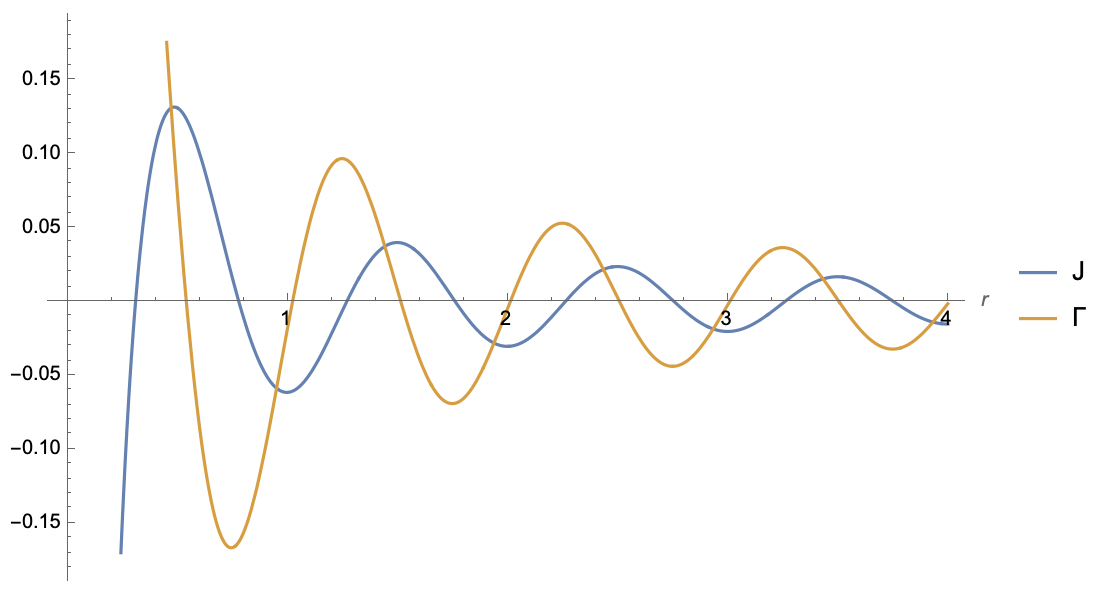
\includegraphics[width=0.4\textwidth]{figures/J_and_Gamma.png} 
    \caption{•}
    \label{fig:J_and_Gamma.png}
\end{figure}
% \commentSB{It might be better if these figures go along with the first figure, at the top of this page}
Into this lattice, we place one or two lattice impurities with transition frequency $\omega_I \approx \omega_L$. The overall Hamiltonian is $H = H_L + H_{LI} + H_{I}$, where $H_L$ is the Hamiltonian of the lattice, $H_{LI}$ is the Hamiltonian for the interaction between the lattice and any impurities, and $H_{I}$ is for the interactions involving just impurities. These Hamiltonians are defined such that  

\begin{subequations}
    \begin{align}   
        H_L = \sum_i^{N_L} \left( \omega_L - \frac{i}{2} \gamma_L \right) \sigma_i^\dag \sigma_i + \sum_{i,j \neq i}^{N_L} \left( J_{ij} - \frac{i}{2} \Gamma_{ij} \right) \sigma_i^\dag \sigma_j \\
        H_{LI} = \sum_{i}^{N_L}  \sum_{j}^{N_I} \left[ \left( J_{ij} - \frac{i}{2} \Gamma_{ij} \right) \sigma_i^\dag s_j + \left( J_{ji} - \frac{i}{2} \Gamma_{ji} \right) s_j^\dag \sigma_i \right] \\
        H_I = \sum_j^{N_I} \left( \omega_I - \frac{i}{2} \gamma_I \right) s_j^\dag s_j + \sum_{i,j \neq i}^{N_I} \left( J_{ij} - \frac{i}{2} \Gamma_{ij} \right) s_i^\dag s_j
        \label{eqn:Hamiltonian}
    \end{align}
\end{subequations}

where $N_L$ is the number of lattice atoms, $\sigma_i$ is the lowering operator for lattice atom $i$, $N_I$ is the number of impurities, and $s_j$ is the lowering operator for impurity $j$. 

% \commentTP{Add impurity Hamiltonian! Write as H = HL + HLI + HII. Define for the two-imputity case, and say that you just take away some terms to get the single impurity case. Write out each of these three terms as three separate equations}

\commentSB{Then, at some point here or later, explain the role of the detuning delta}

%==============================================================================================
\section{Single impurity case}
\commentSO{Define lattices, define distances related to lattices, $\Gamma_\mathrm{eff}$, constant area}

% \commentTP{Remember to say that we only focus on non-centered Bravais lattices, never centered Bravais lattices. }

% \commentSB{Put the self-energy calculation here, along with the Gamma-eff calculation? Because I don't think there's anything more to say here. Any details about the geometries need to be left to the specific sections directly below here.}

The generic form of the Hamiltonian for a given lattice of $N$ atoms along with a single impurity is 

% \begin{equation}
%     H = \begin{pmatrix}
%         H_{11} & H_{12} & \cdots & H_{1N}  &  C_{LI,1}\\ 
%         H_{21} & H_{22} & & H_{2N}         & C_{LI,2} \\
%         \vdots & & \ddots & \vdots         & \vdots  \\
%         H_{N1} & H_{N2} & \cdots & H_{NN} & C_{LI,N} \\
%         C_{IL,1} & C_{IL,2} & \cdots & C_{IL,N} & H_I   
%     \end{pmatrix}
% \end{equation}
\begin{equation}
    H = \begin{pmatrix}
        ~ & ~ & ~ &   C_{LI} \\ 
        ~ & H_L & ~ & \vdots \\
        ~ & ~ & ~ & C_{LI} & \\
        C_{IL} & \cdots & C_{IL} & H_I   
    \end{pmatrix}
    \label{eqn:blockH1}
\end{equation}
where $H_L$ represents the $N \times N$ matrix of terms for the lattice's own Hamiltonian, $H_I$ is the lattice, and $C_{IL}$ along with $C_{LI}$ represent the coupling terms between the lattice atoms and the impurity. 
% \commentSB{Firstly, is there some better notation than this, especially $C_{IL,1}$, with that comma there. Secondly, does $C_{IL,1} = C_{LI,1}$, or is there some other symmetry that can be exploited in the notation?}

Define the wavefunction such that
$ \psi = 
\begin{pmatrix}
    b_1 && \vdots && b_N && c
\end{pmatrix}^T 
\label{eqn:psi} $,
and assume that the lattice occupies a steady state, so that the Schr\"odinger equation is

\begin{equation} i \hbar 
    \begin{pmatrix}
    0 \\ \vdots \\ 0 \\ \dot{c}
    \end{pmatrix} = \begin{pmatrix}
        ~ & ~ & ~ &   C_{LI} \\ 
        ~ & H_L & ~ & \vdots \\
        ~ & ~ & ~ & C_{LI} & \\
        C_{IL} & \cdots & C_{IL} & H_I   
    \end{pmatrix} \begin{pmatrix}
        b_1 \\ \vdots \\ b_N \\ c
    \end{pmatrix} 
\end{equation}
This can be solved to get 
\begin{equation}
    \begin{pmatrix}
        b_1 \\ \vdots \\ b_N
    \end{pmatrix} = - H_L^{-1} C_{LI} c
\end{equation}
Putting this back into the Schr\"odinger equation produces 
\begin{equation}
    \dot{c} = -i (H_I - C_{IL}^T H_L^{-1}C_{LI}) c
\end{equation}
Recognizing that $ H_I - C_{IL}^T (H_L^{-1}) C_{LI} = \Sigma_I - i \frac{\gamma_I}{2} $, we can calculate the impurity's self-energy $\Sigma_I$ to be 
% \commentSB{Should this identification be justified?}
\begin{equation}
    \Sigma_I = H_I - C_{IL}^T (H_L^{-1}) C_{LI} + i \frac{\gamma_I}{2}
    \label{eqn:selfenergy}
\end{equation}
The effective decay rate $\Gamma_\text{eff}$ for an impurity in the lattice is related to this self-energy according to 
\begin{equation}
    \Gamma_\text{eff} = \gamma_I - 2~\im[\Sigma_I]
\end{equation}

\begin{figure}
    \centering
    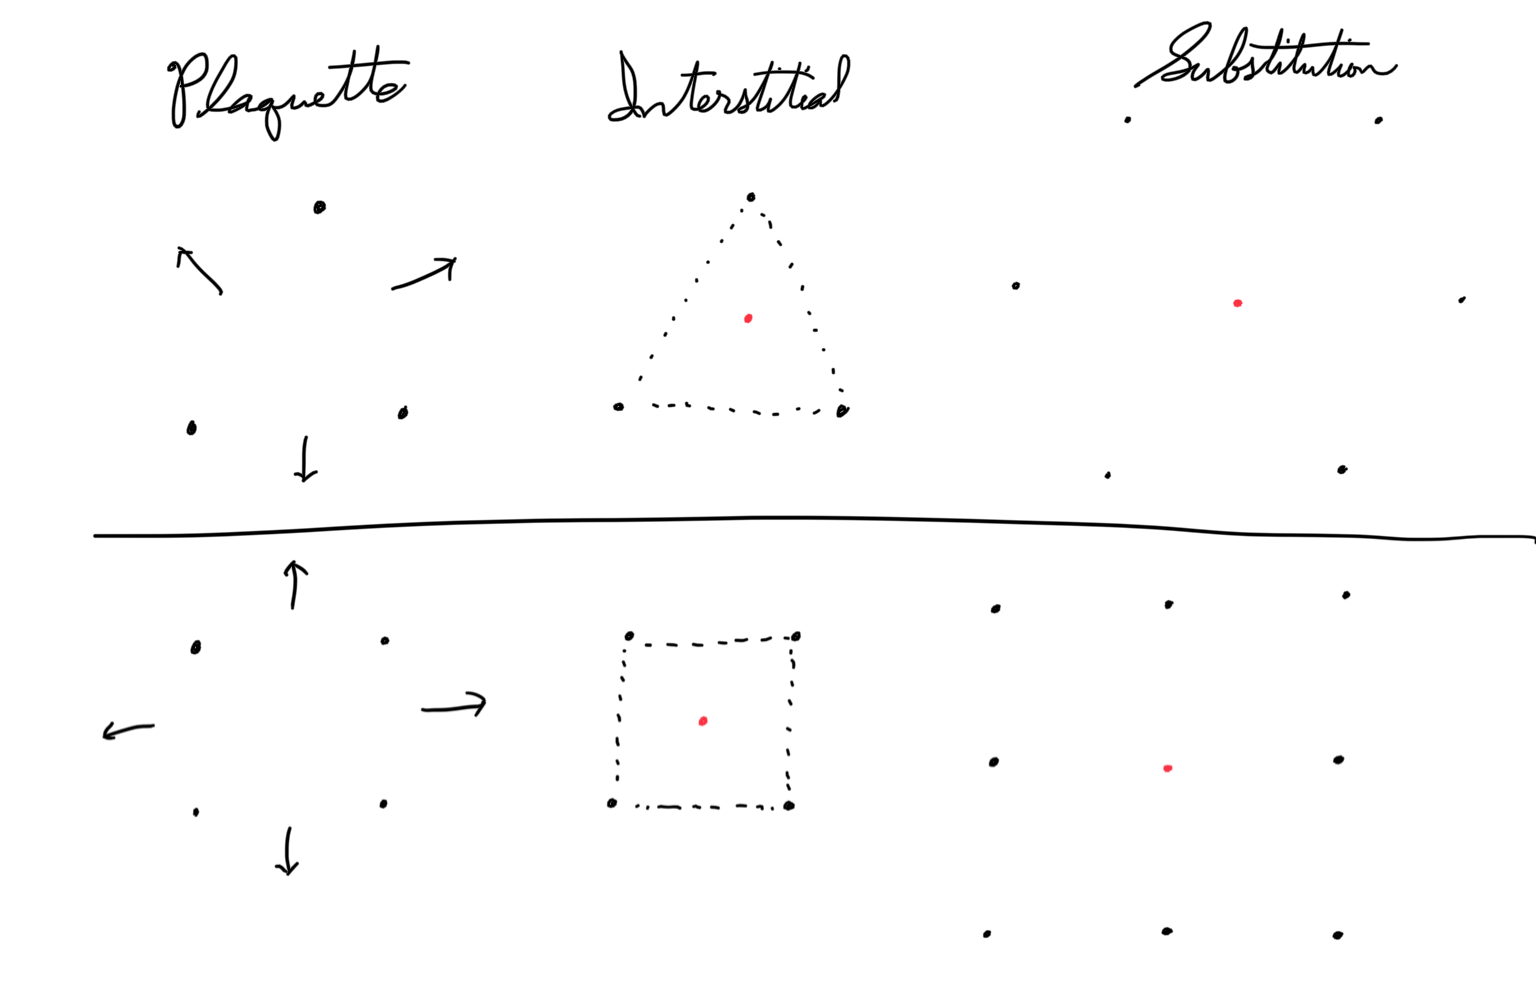
\includegraphics[width=0.4\textwidth]{figures/triangle_and_square.png} 
    \caption{•\commentSB{Should this be made into one long line and put at the top of a page? Also, maybe draw out the full lattices, all 4x4, and the whole triangular lattice. Or maybe just the triangular lattice?}}
    \label{fig:Bravais}
\end{figure}

Equipped with these mathematical tools, we consider the full range of non-centered Bravais lattices, for both interstitial and substitutional impurity positions, as illustrated in \fref{fig:Bravais}. In order to reasonably compare lattices of differing geometries, we ensure, whenever possible, that all plaquettes possess the same area throughout all possible transformations. 

% , because...
% \commentSB{Does this argument rely on a momentum-space view of things? In any case, make this constant area argument rigorous}

------------------------

\commentSB{This is just a holding space for this matrix, in case we want to copy and paste it to anywhere. I don't actually intend for it to sit here in this section.}

\begin{equation}
    H = 
    \begin{pmatrix}
        -\frac{i \gamma_L}{2} - \frac{\delta_{LI}}{2} & J(r_{12}) - \frac{i \Gamma(r_{12})}{2} & \cdots \\
        J(r_{21}) - \frac{i \Gamma(r_{21})}{2} & -\frac{i \gamma_L}{2} - \frac{\delta_{LI}}{2} & & \\
        \vdots & & \ddots
    \end{pmatrix}
\end{equation}

\subsection{Interstitial}

\begin{figure*}
    \centering
    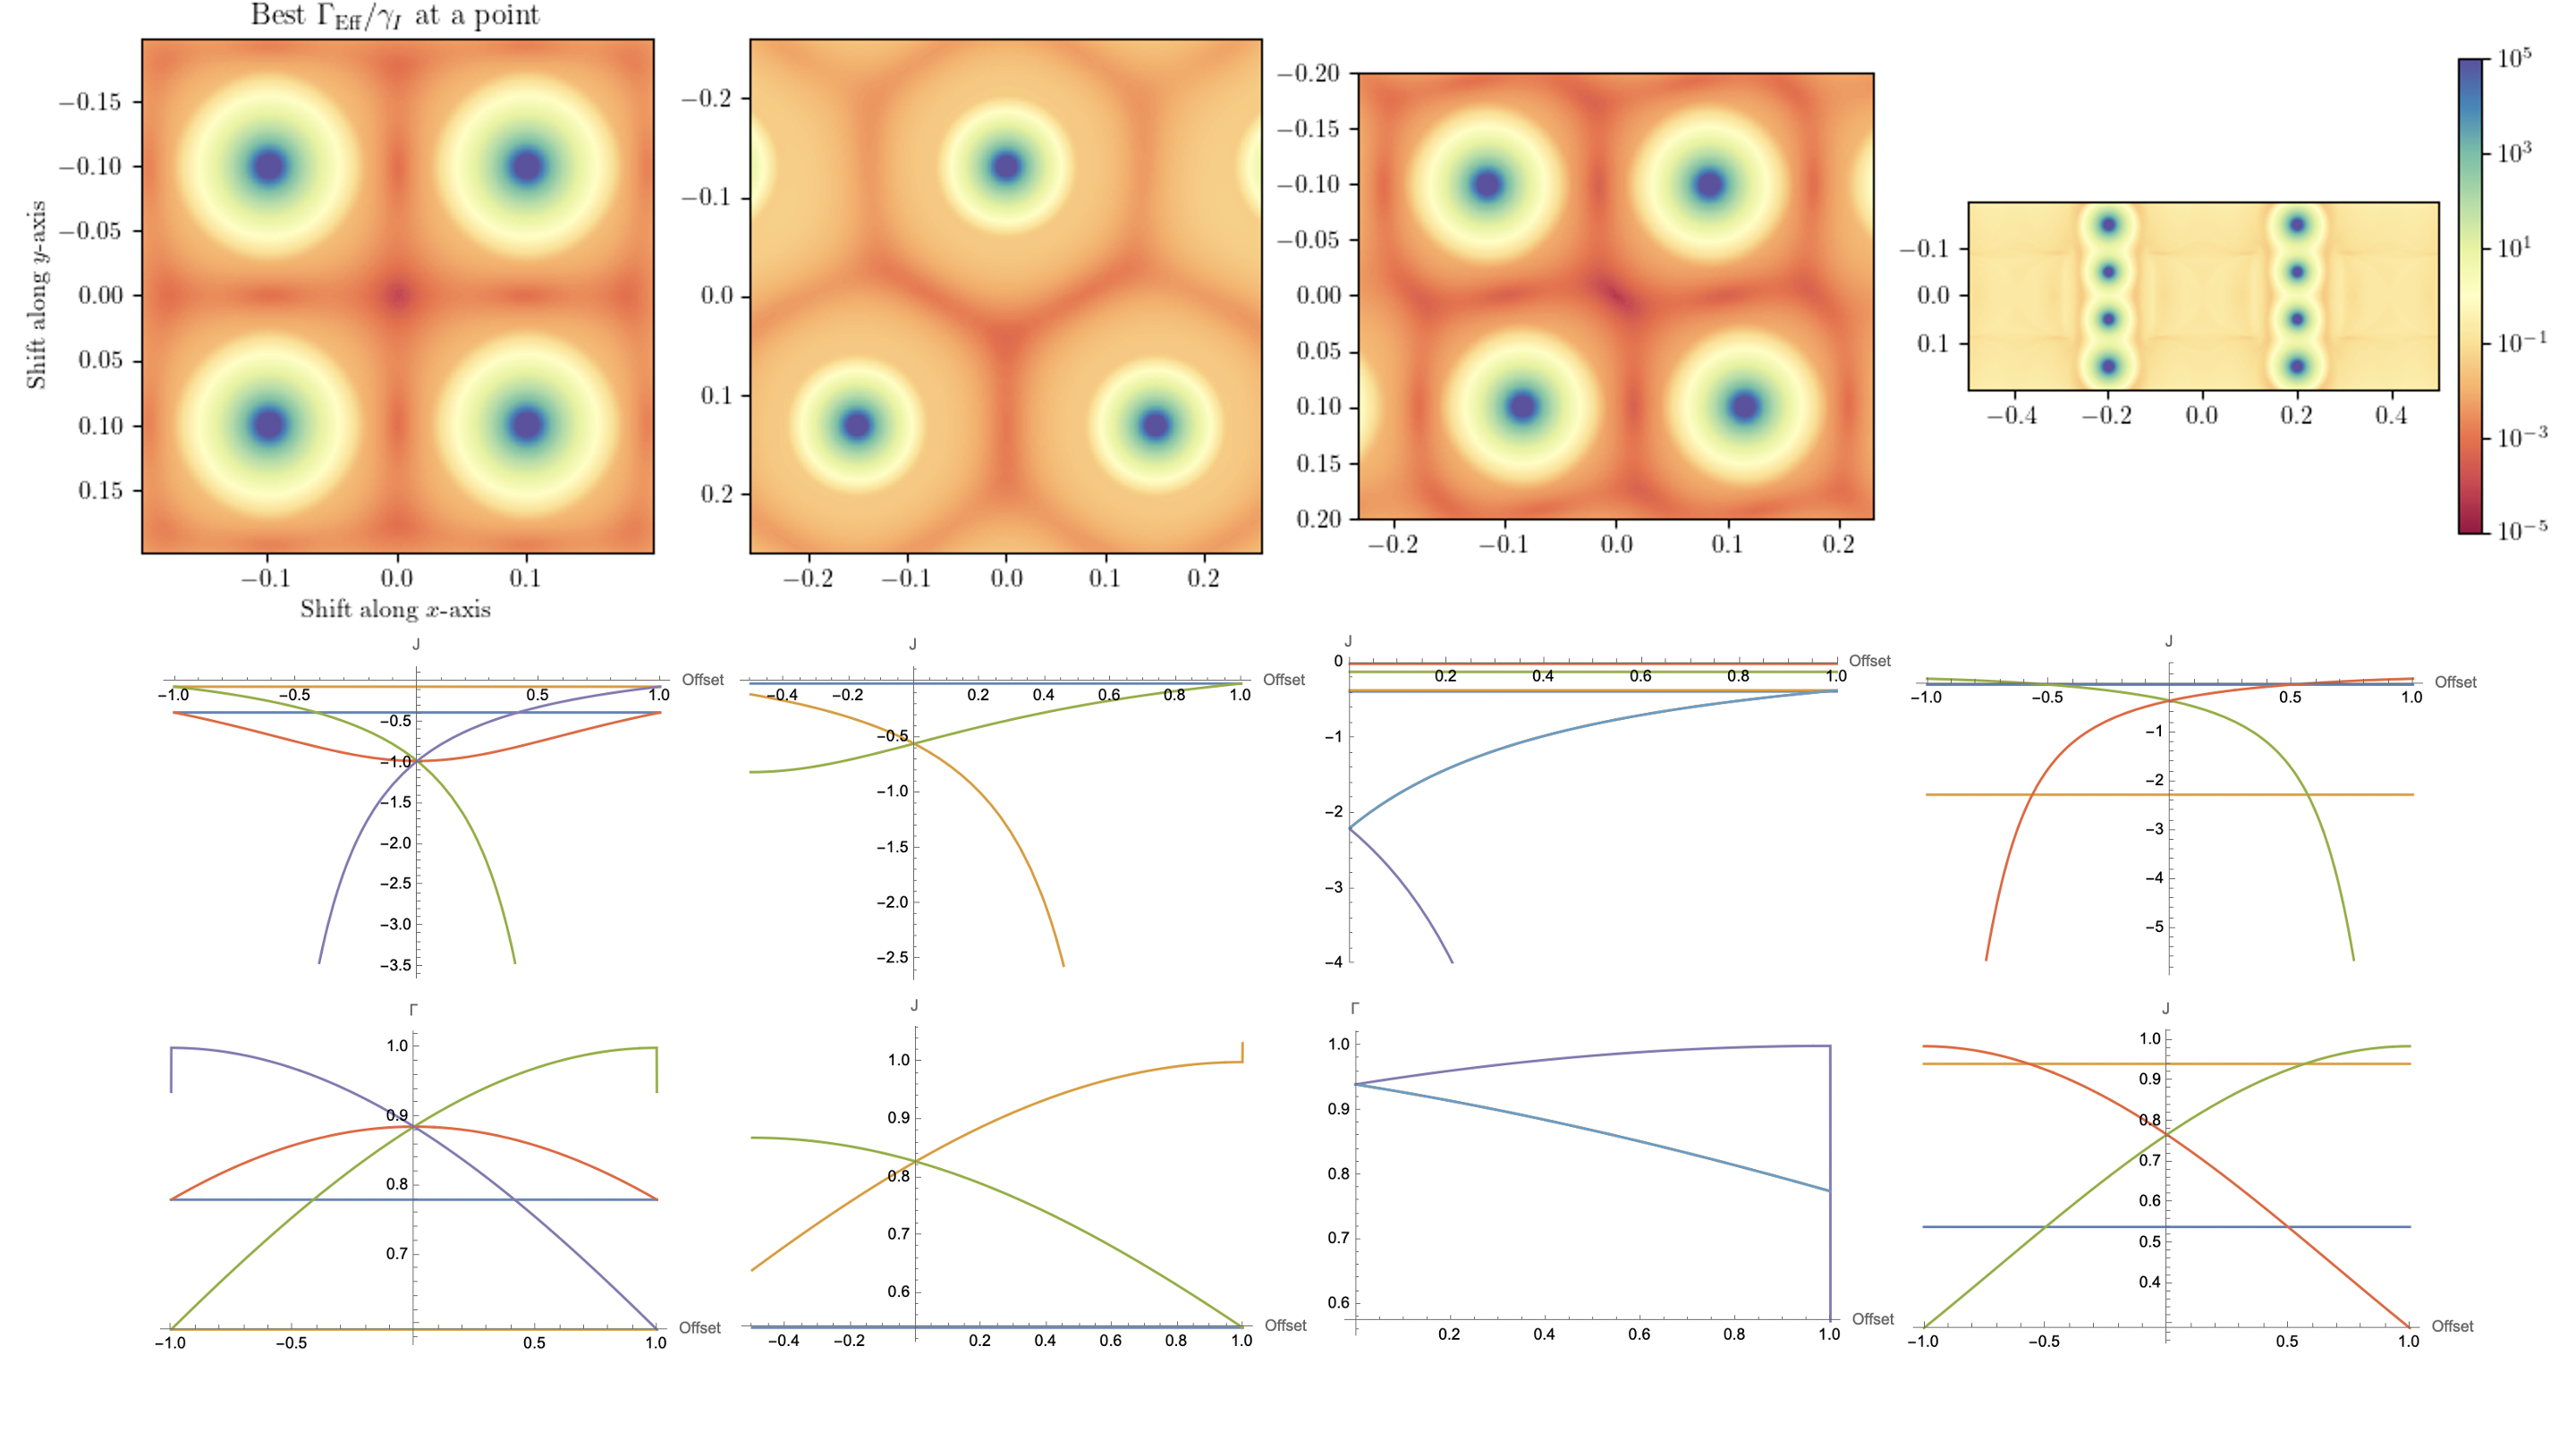
\includegraphics[width=1.0\textwidth]{figures/interstitial_figure.png} 
    \caption{•\commentSB{To do: 1) Change monoclinic plaquette to something more like theta = 0.4.   2) Change rectangular scaling to something more like 1.5   3) Draw line paths across all the plaquettes, illustrating which paths the plots are graphed over}}
    \label{fig:interstitial}
\end{figure*}

Consider a finite square lattice, with an inter-atomic spacing of $a = 0.2$, defined as a function of the lattice's resonant wavelength. Compare this to the other Bravais lattices, namely a triangular lattice, and monoclinic lattice defined over $\theta$ from $\pi/2$ to $0$, and a rectangular lattice with a scaling factor $\mu$ such that the horizontal sidelength of its rectangular plaquette is $\mu a$. 
\commentSB{Which variable do we want for scaling? Does $\mu$ work?.} To ensure that the plaquettes of all of these lattices have the same area, we set the sidelength of the triangular plaquettes to $\frac{2}{3^{1/4}}a$, the height of monoclinic lattices to $a$ for all $\theta$, and the height of the rectangular lattices to $a/\mu$. 

For an interstitial impurity, the position of the impurity in the plaquette along with its detuning relative the lattice's resonant frequency determine its decay properties. Detuning is defined as $ \delta_{LI} = \omega_I - \omega_L$. For a given impurity position, $\delta_{LI}$ can be chosen to give optimal $\Gamma_\text{eff}$, by minimizing along a curve such as \fref{fig:delta_check}. By conducting this optimization for all positions within a plaquette, a map of the optimal impurity placement can be constructed. The results of this are depicted in \fref{fig:interstitial}. See the appendix for the values of $\delta_{LI}$ corresponding to these impurity positions. 

In all cases, geometric symmetries determines where the points of minimal $\Gamma_\text{eff}$ lie. The paths of minimal $\Gamma_\text{eff}$ follow the geometry of a Voronoi diagram where the lattice atoms are taken to be ... 



Whichever geometry one examines, the center of the plaquette is either the optimal position, or at least one of the better positions. For highly symmetric lattices, such as the square lattice and the triangular lattice, it is unequivocally the optimal position, while for lattices where some symmetries are broken by a variable paramter, such as the monoclinic and rectangular lattices, other points can have slower decay rates than the center. 

The role of symmetry is particularly clear once the coupling terms between pairs of particles are plotted over paths through the plaquette space. 

In particular, the points at which the values of coupling terms coincide match the points of geometric symmetry. This is to be expected, 

(as with a square lattice and a triangular lattice)

(as with the monoclinic lattice and the rectangular lattice)

\fref{fig:interstitial} depicts the optimal value of $\Gamma_\text{eff}$


\begin{figure}
    \centering
    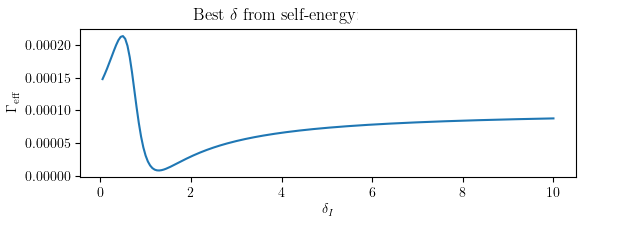
\includegraphics[width=0.4\textwidth]{figures/temp_delta_check_cropped.png} 
    \caption{•}
    \label{fig:delta_check}
\end{figure}







\subsection{Substitutional}


\subsection{Square vs. triangular}

Consider a finite square lattice, with an inter-atomic spacing of $a = 0.2$, defined as a function of \commentSB{that characteristic wavelength}. 

Compare this to a triangular lattice with the same plaquette area, and hence, a side-length of (...) 
\commentSB{fill in these details}
% \commentSB{see earlier point about how we should really use constant area}

% \begin{figure}
%     \centering
%     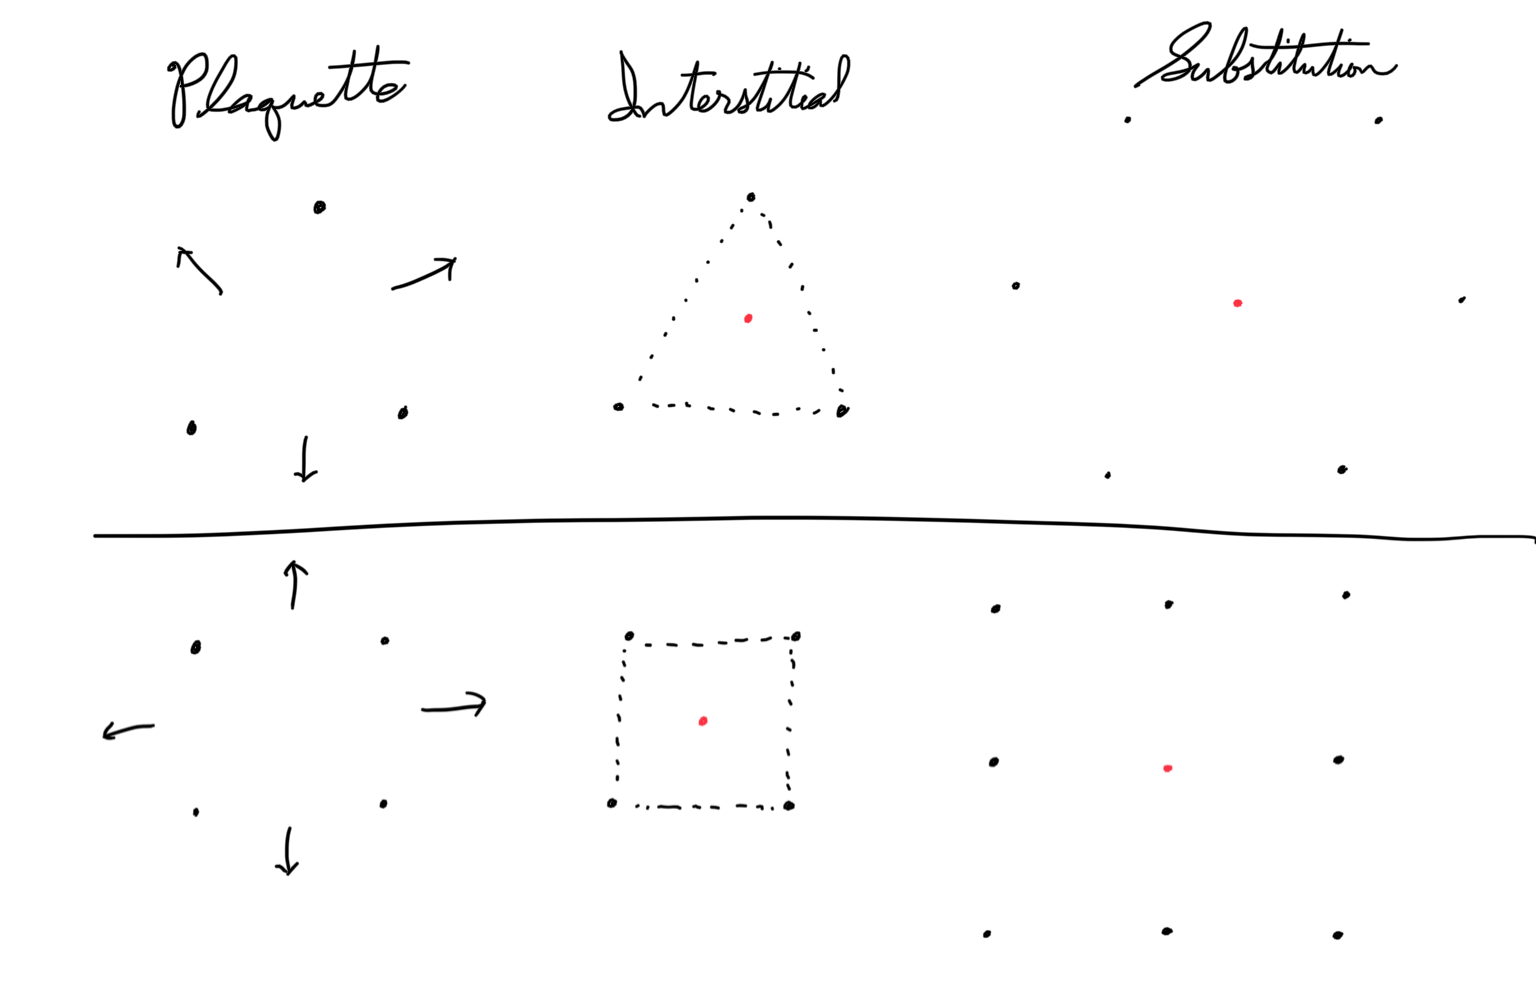
\includegraphics[width=0.4\textwidth]{figures/triangle_and_square.png} 
%     \caption{•\commentSB{Should this be made into one long line and put at the top of a page? Also, maybe draw out the full lattices, all 4x4, and the whole triangular lattice. Or maybe just the triangular lattice?}}
%     \label{fig:Bravais}
% \end{figure}

\commentSB{Put a diagram of all the Bravais lattices, as a part of this one.}

See \fref{fig:Bravais}.

% \commentTP{Put a figure that just shows a single plaquette for each of our two cases here, with dots going off in 4 and 3 directions respectively}

%=================
\subsubsection{Interstitial}
\commentSO{Interstitial which imposes one more length scale -> refer to analytics, numerics -> impurity position}
Now, consider an impurity atom placed within a plaquette. For the square case, we implemented this arrangement using a $4\times 4$ lattice, so that the impurity was centered within the lattice. 

% \commentSB{Put a small diagram here? You can illustrate the length scales here as well}

Likewise, for the triangular case, we placed the impurity at the center of a \commentSB{12 atom?} lattice, with the following arrangement. 

% \commentSB{diagram?}

By placing the impurity at the center of a plaquette, only one additional length scale is introduced. 
%  Hence, the coupling as a function of inter-atomic spacing is \commentSB{fairly constant, looking at the analytics?} 

% \commentSB{J and Gamma diagrams}

% \commentSB{Should we vary inter-atomic spacing?}

After attempting to place the impurity off-center, 

% \commentTP{Have a plot of Gamma over delta, to justify how we choose an "optimum" delta}

% \begin{figure}
%     \centering
%     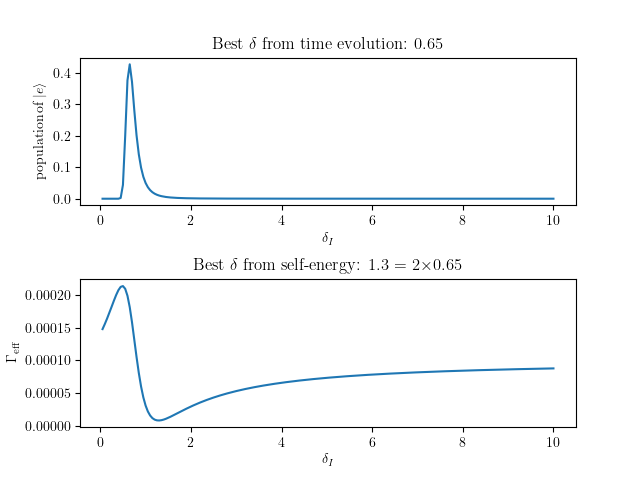
\includegraphics[width=0.4\textwidth]{figures/delta_check.png} 
%     \caption{•}
%     \label{fig:delta_check}
% \end{figure}

% \begin{figure}
%     \centering
%     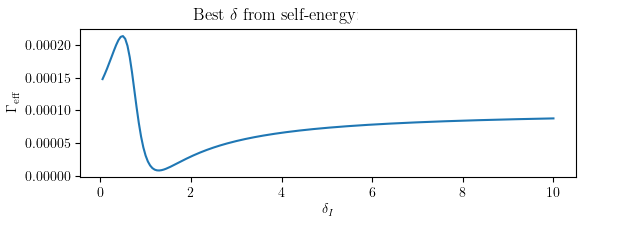
\includegraphics[width=0.4\textwidth]{figures/temp_delta_check_cropped.png} 
%     \caption{•}
%     \label{fig:triangle_and_square_plaquette_interstitial}
% \end{figure}

\commentSB{Either one or both of these plots, perhaps for some different range of values. Also, can this be fully in-line, or shoud it be given a caption?}
\commentTP{Have a single graph, from the analytics}

% \commentSB{numerics plaquette plots}
\begin{figure*}
    \centering
    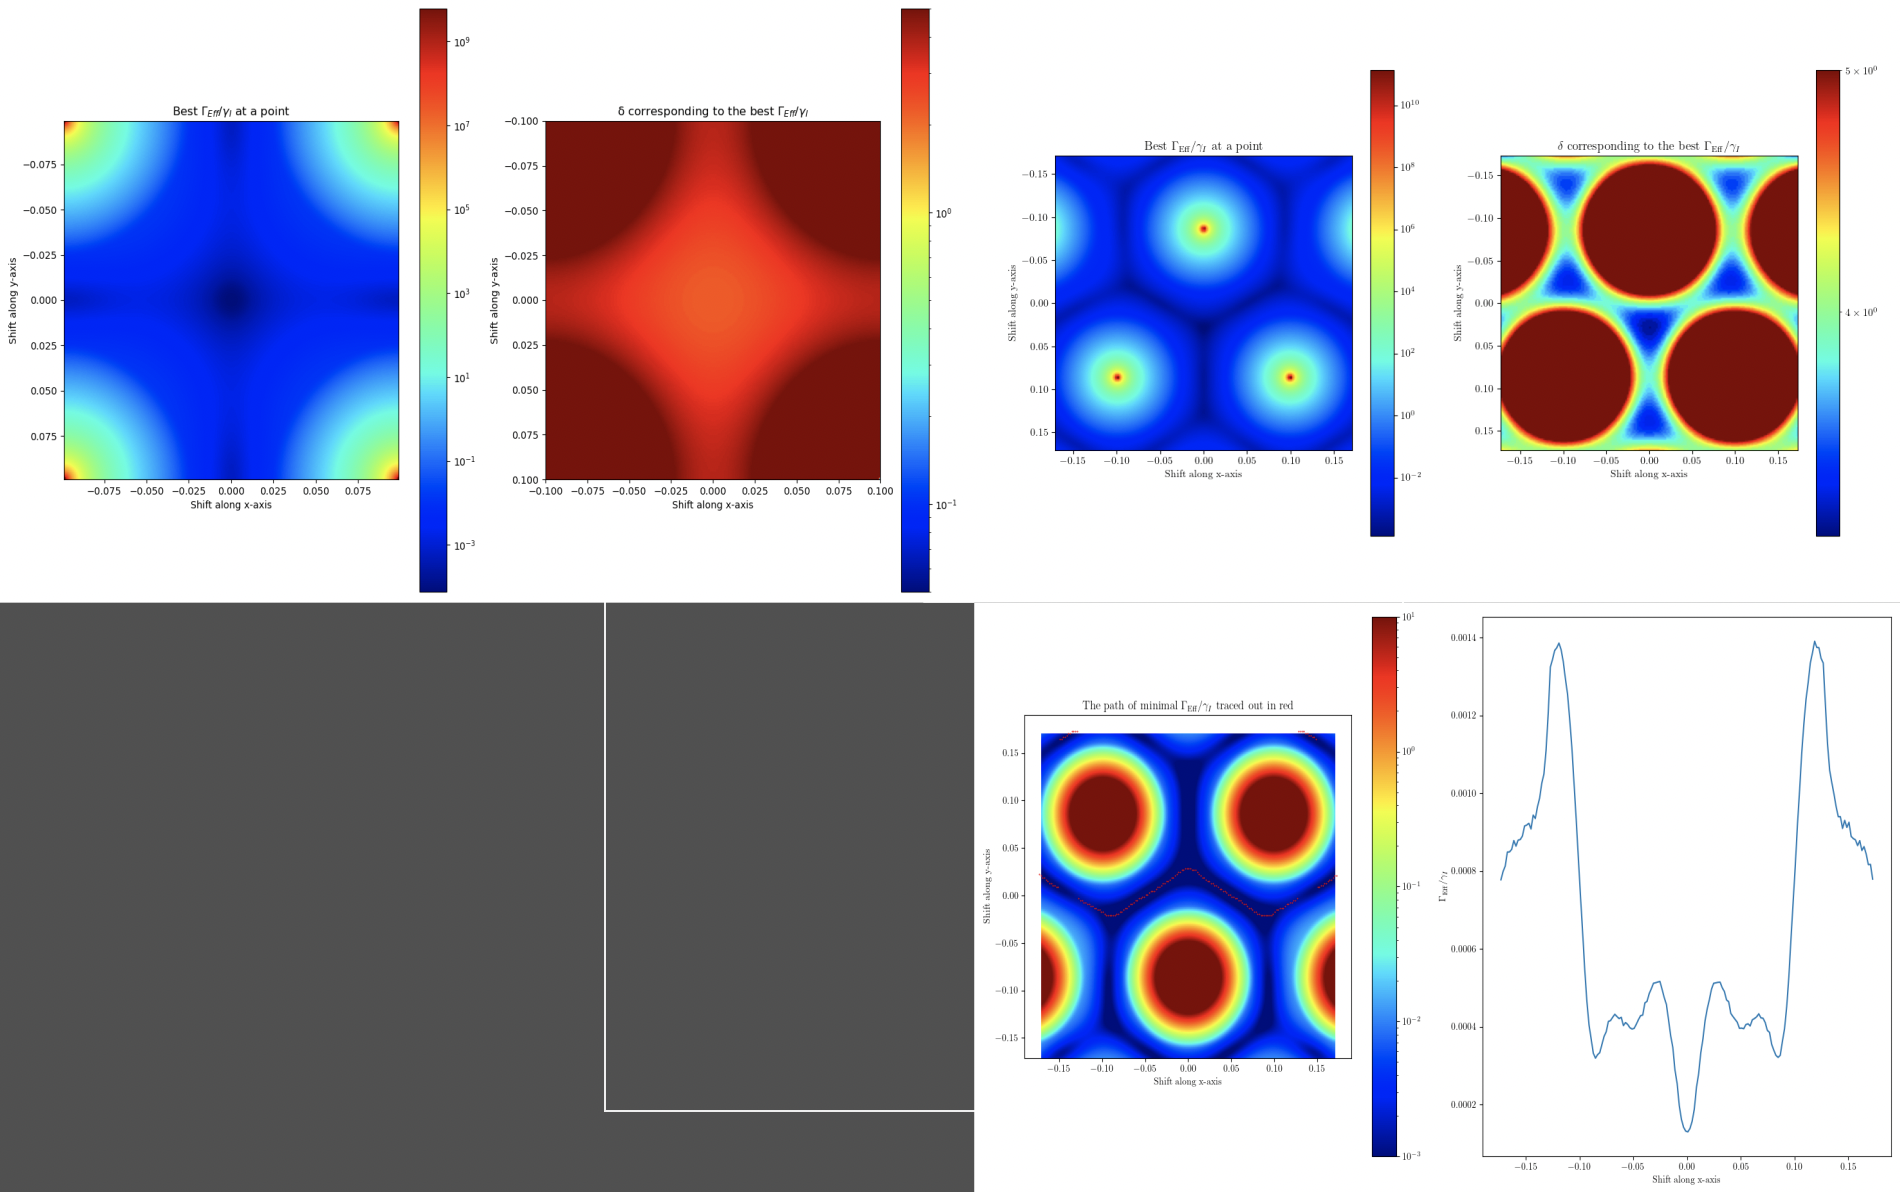
\includegraphics[width=1.0\textwidth]{figures/triangle_and_square_plaquette_interstitial.png} 
    \caption{•}
    \label{fig:triangle_and_square_plaquette_interstitial}
\end{figure*}
\commentSB{Should the plots in \fref{fig:triangle_and_square_plaquette_interstitial} and \fref{fig:triangle_and_square_plaquette_substitution} be separate?}
\commentTP{Take out optimal delta values, and put it in the appendix. Change to Stefan's reccomendation, with square and triangle side-by-side, and the minimal lineplots directly below}

it is clear that the point at which the impurity atom experiences minimal decay is at the center of the plaquette. 

% \commentSB{plaquette lineplots showing minimal Gamma}

This point also possesses the highest symmetry, suggesting that additional symmetries lead to slower decay rates. This hypothesis is supported by the behavior of the coupling constants for various positions of the impurity away from the center 

\commentSB{a diagram of this description, which has not been made yet. Or perhaps two diagrams, one moving from the center to a lattice point, and another moving from the center to the midpoint between two lattice points. Actually, four diagrams, because these two should be made for both the square and triangular cases. See placeholder below}

% \begin{figure}
    % \centering
    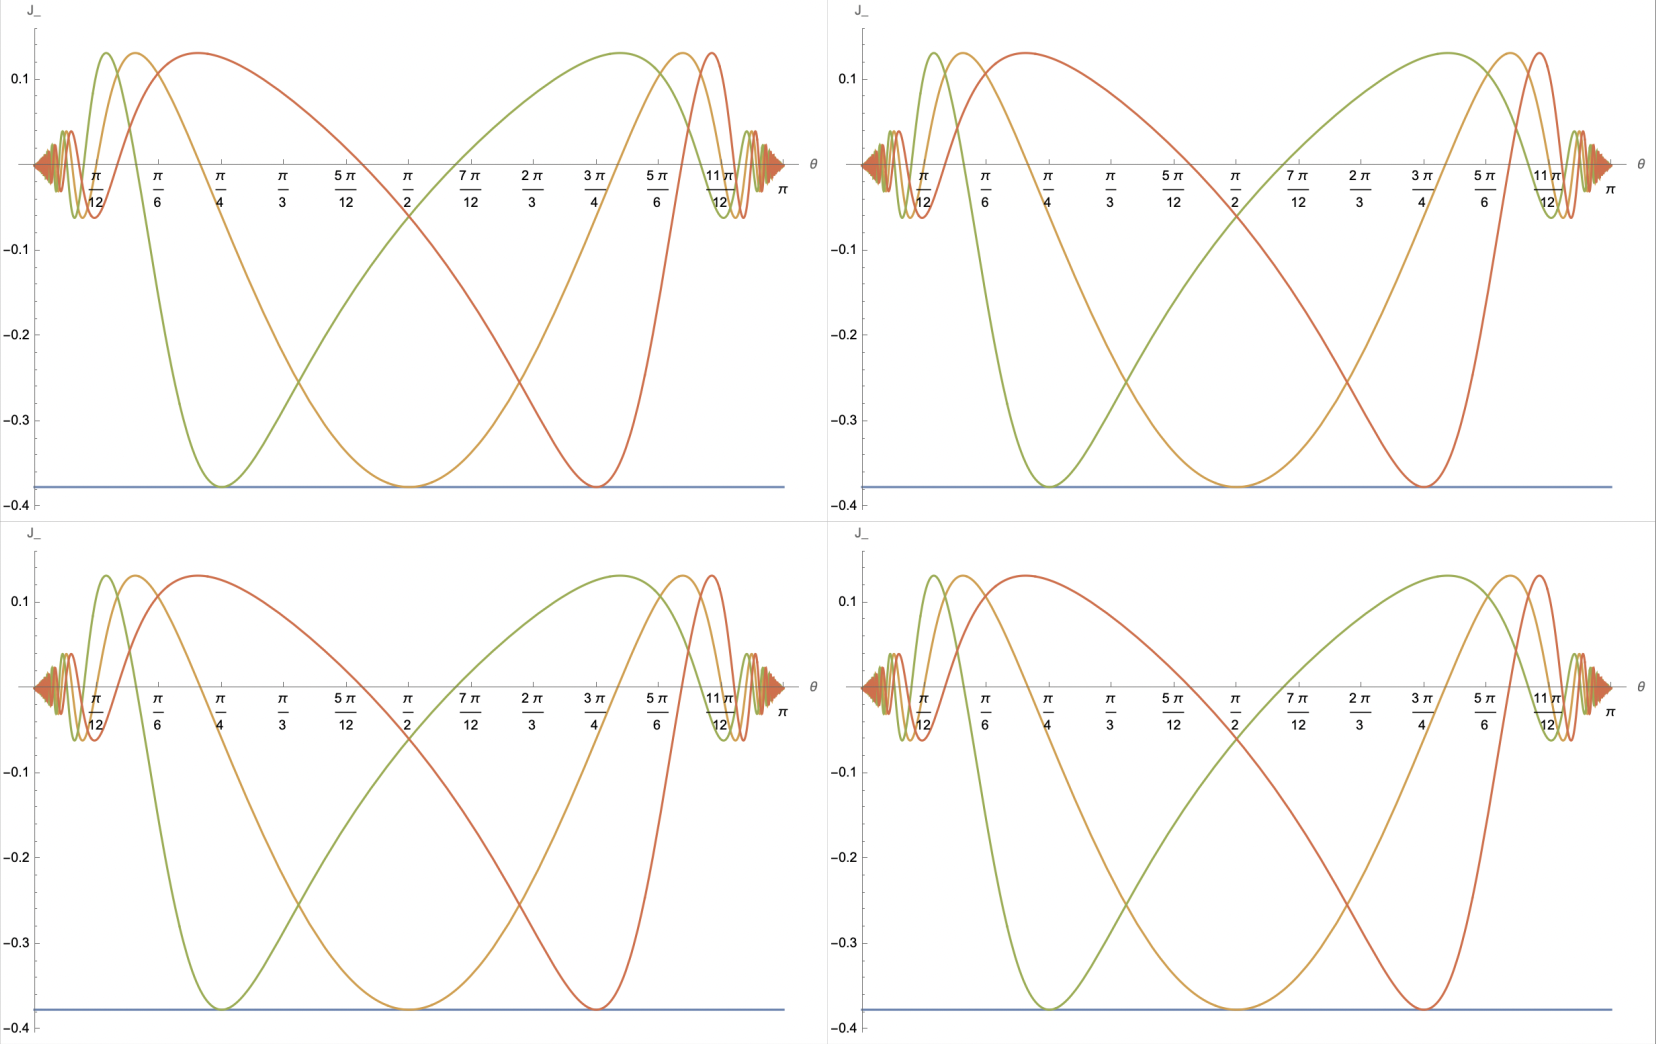
\includegraphics[width=0.4\textwidth]{figures/triangle_and_square_interstitial_coupling.png}
    % \label{fig:triangle_and_square_coupling}
% \end{figure}


\commentSB{This is a placeholder. again, should this be given a caption?}
\commentTP{Consolidate into the two big pictures of this section, as Stefan's outline shows}


%=================
\subsubsection{Substitution}
\commentSO{Does NOT(!) impose another length scale as long as it is not away from the center -> refer to analytics, -> always at band edge, numerics -> impurity position}

Now, considering substituting a lattice atom for an impurity, so that, in effect, the impurity takes up a vacancy in the lattice. For the square lattice, we used this $5 \times 5$ geometry for our analysis:

\commentSB{diagram. Or is this unnecessary? Probably not}

and for the triangular lattice, we used this geometry

% \commentSB{probably an 18 atom lattice?}
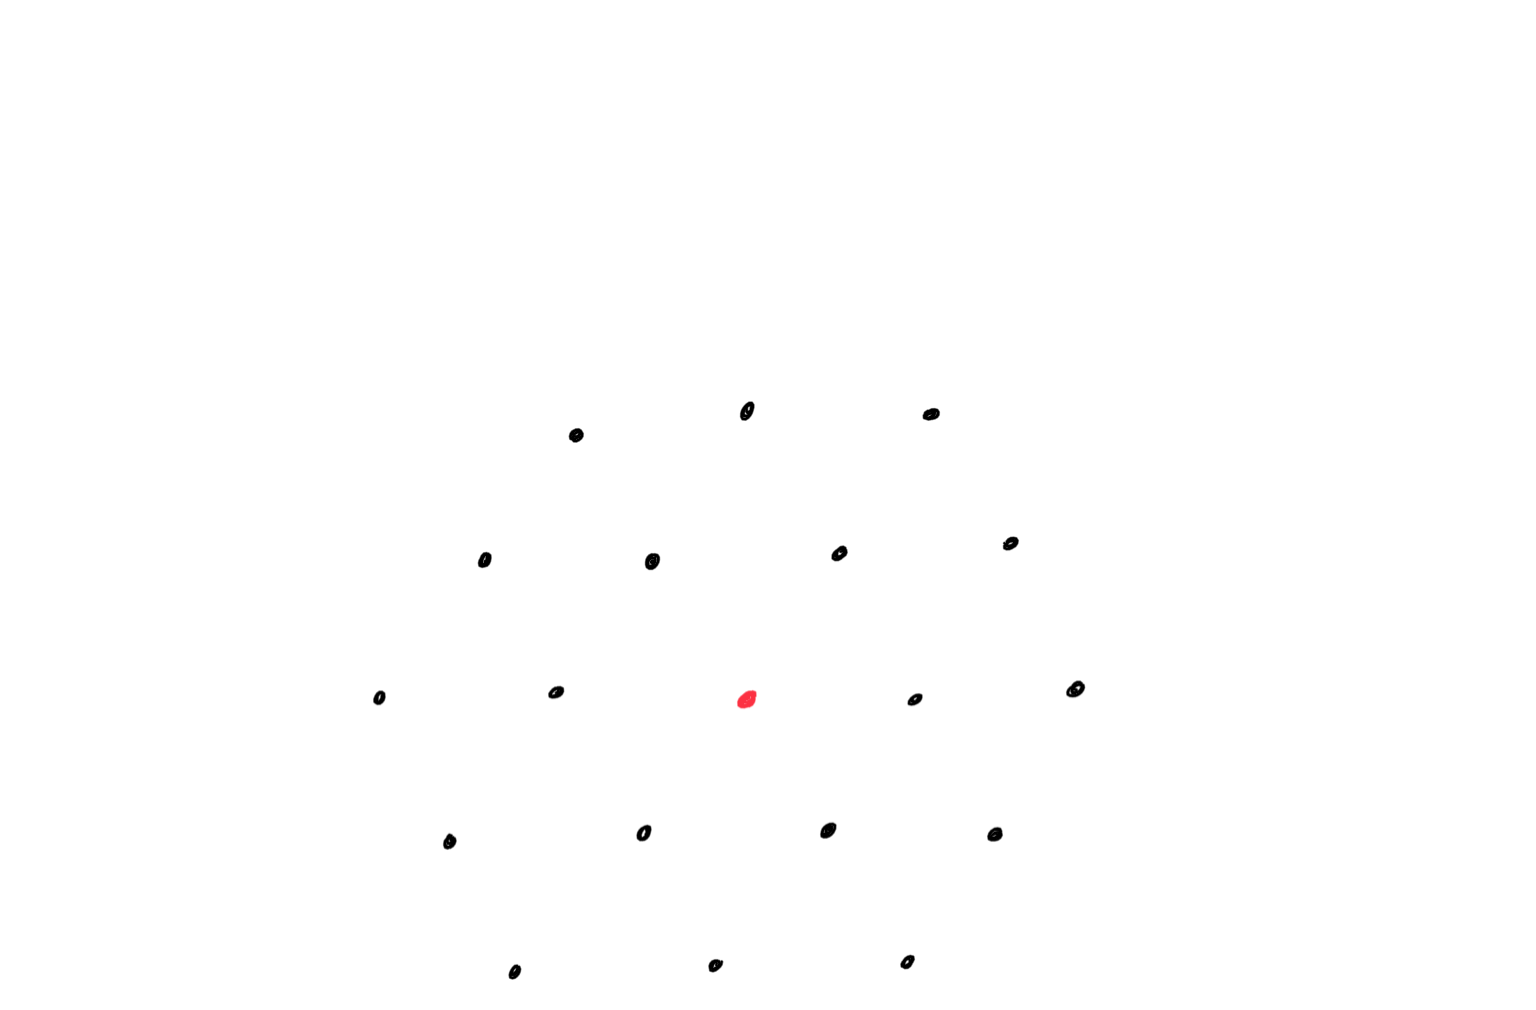
\includegraphics[width=0.4\textwidth]{figures/triangle_substitution_geometry.png}
\commentSB{Don't mind the spacing error, that will be fixed. Also, caption or not? Also, make sure to redo simulations with specifically this geometry}

Performing this substitution on the lattice introduces no additional length scales, as long as the impurity is placed at the center of the vacancy. If it is placed off-center, the best possible values of $\Gamma_\text{eff}$ are 

% \commentSB{plaquette plots from numerics}

\begin{figure*}
    \centering
    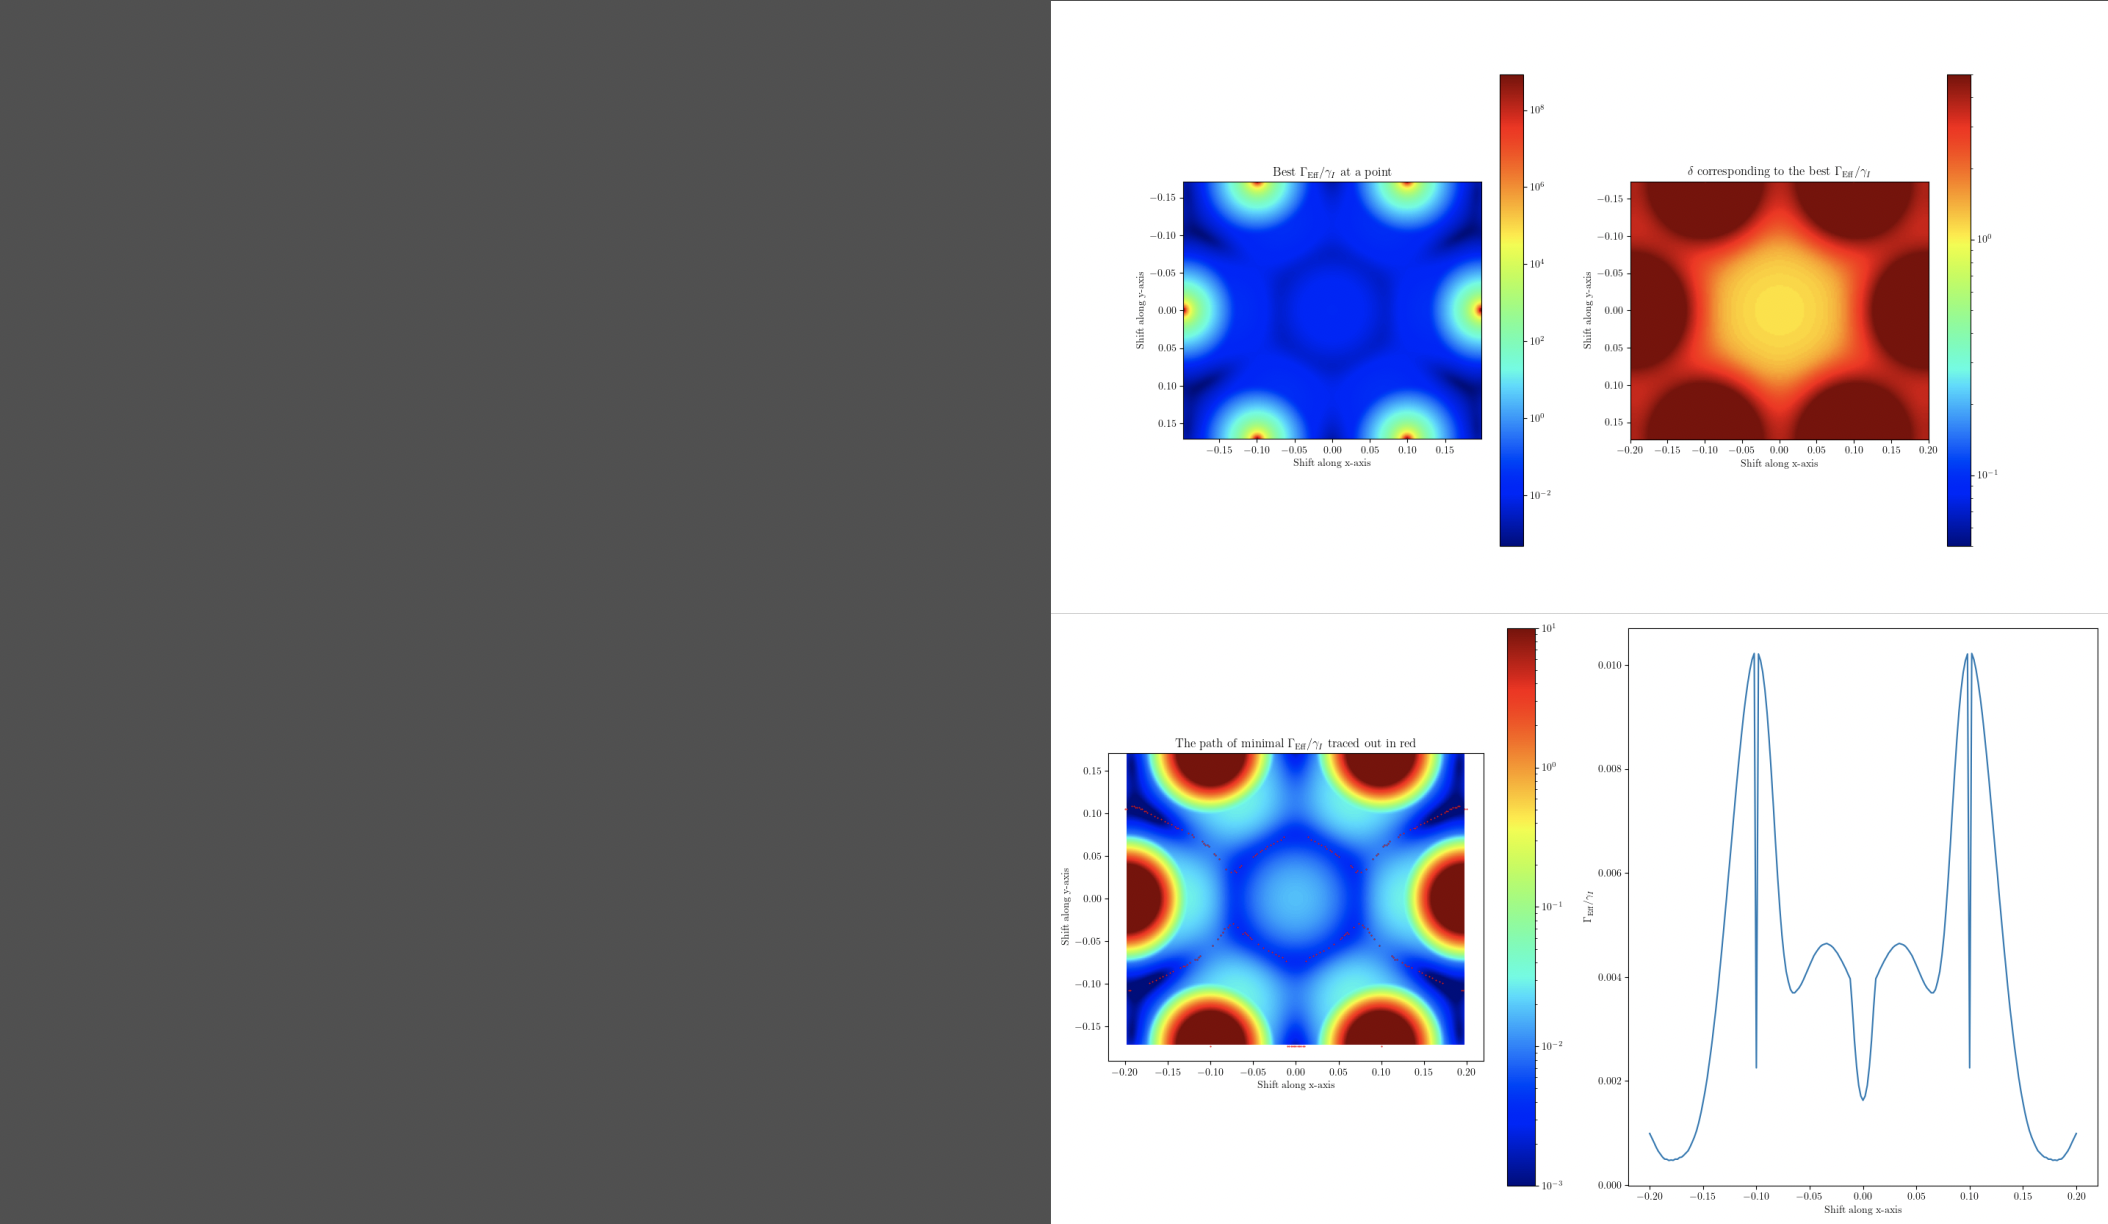
\includegraphics[width=1.0\textwidth]{figures/triangle_and_square_plaquette_substitution.png} 
    \caption{•}
    \label{fig:triangle_and_square_plaquette_substitution}
\end{figure*}

Once again, the point with the highest symmetry experience minimal decay rates.

% \commentSB{plaquette lineplots showing minimal Gamma}

\commentSB{Maybe include another analytic plot showing how symmetry changes coupling constants? Just do this for square lattice.}

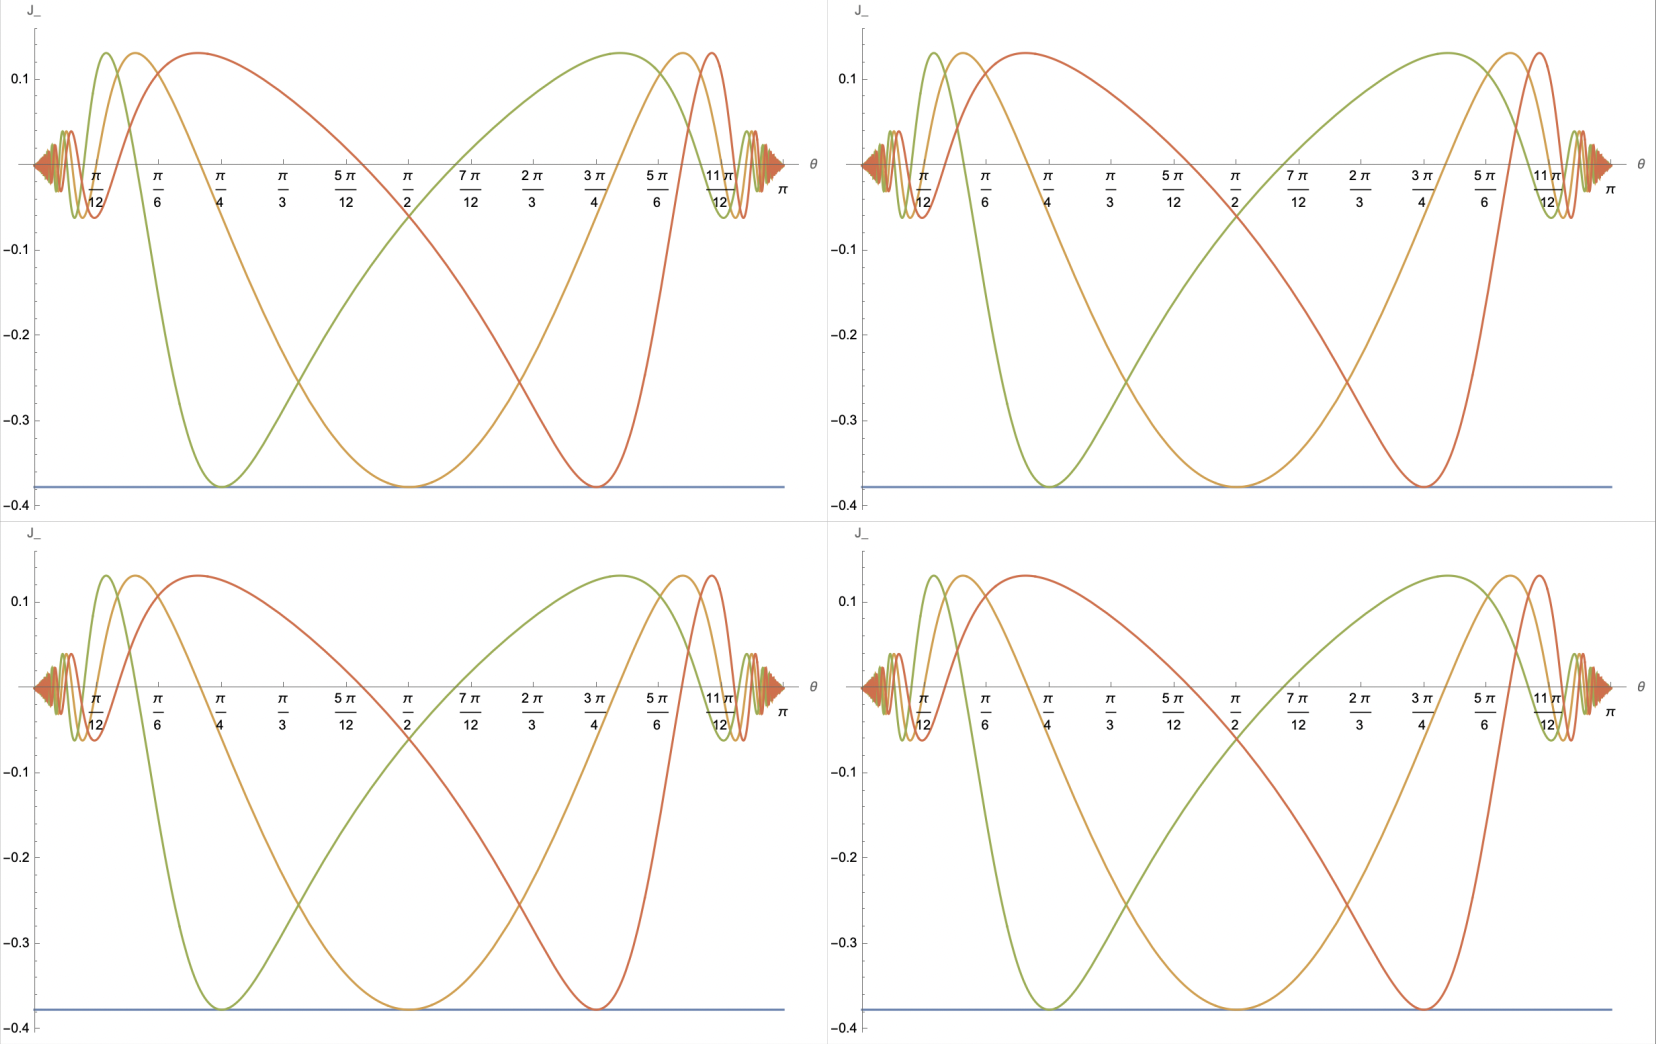
\includegraphics[width=0.4\textwidth]{figures/triangle_and_square_substitution_coupling.png}

\commentSB{placeholder. Also, should this be combined with the other couplings plot? To give a kind of plot of symmetries? Then there will be 3 pages of large plots.}

%==============================================================================================
\subsection{Monoclinic vs. rectangular lattice}
\commentSO{similar arguments}

Now, consider the Bravais lattices defined by variable paramters. 

In particular, consider a monoclinic lattice defined by $\theta$, such that at $\theta = \frac{\pi}{2}$ we recover the square lattice case with an inter-atomic spacing of $0.2$. By maintaining a constant vertical distance between the layers of the lattice, we ensure that the area of the plaquettes remains constant over the range $ 0 < \theta \leq \frac{\pi}{2}$. 

\commentSB{diagram of this geometry}

\begin{figure*}
    \centering
    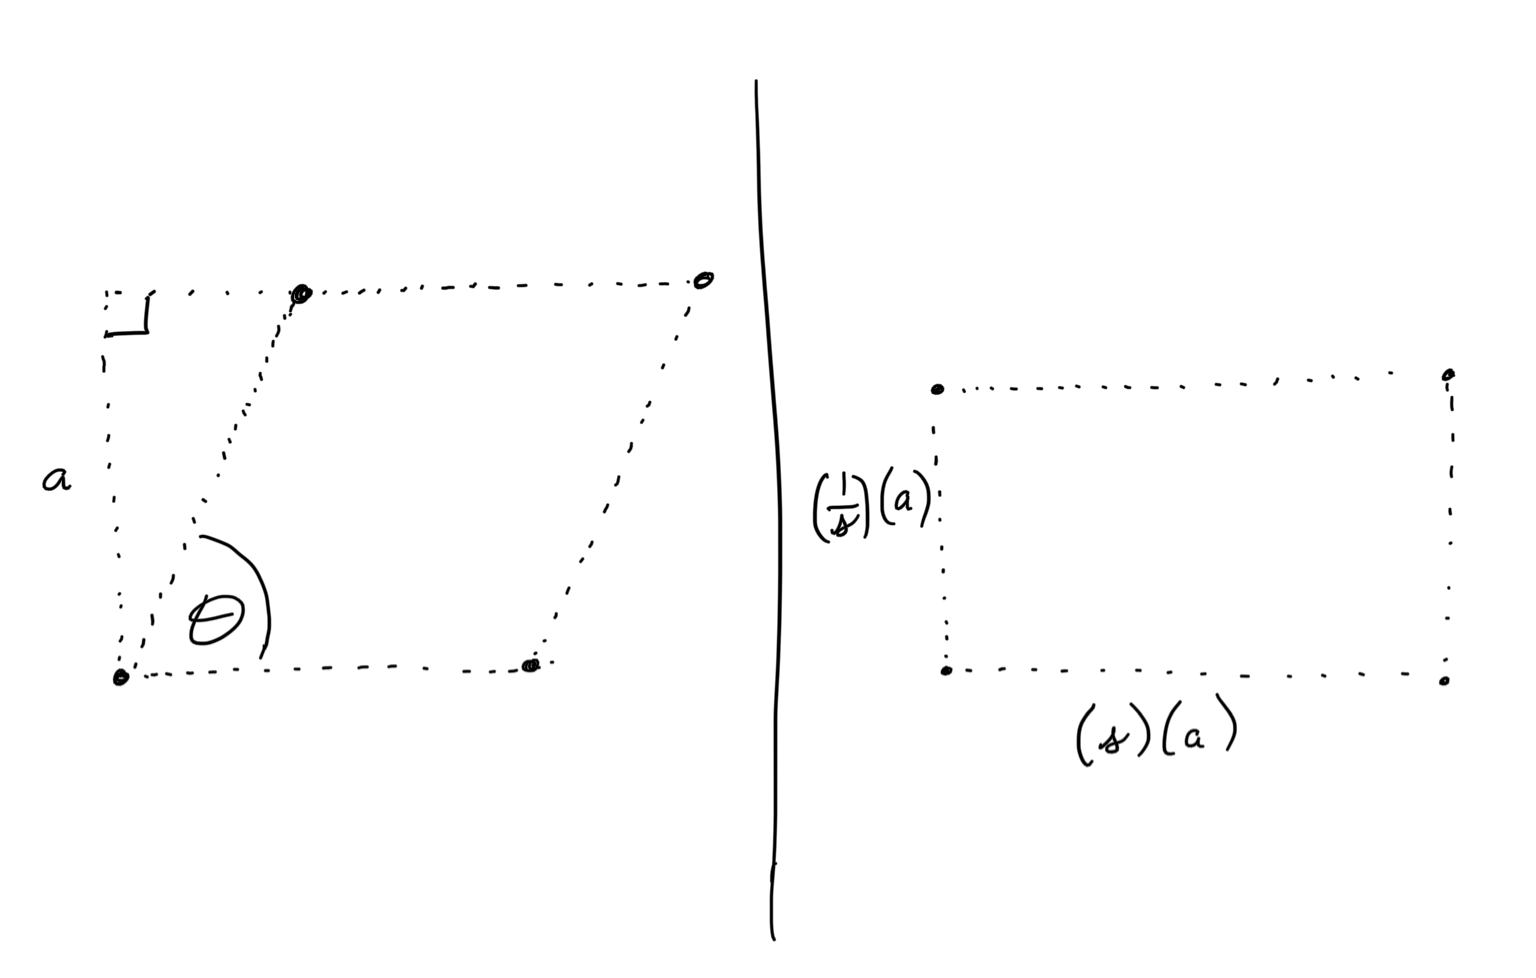
\includegraphics[width=0.4\textwidth]{figures/mono_rect_geo.png} 
    \caption{•}
    \label{fig:mono_rect_geo}
\end{figure*}

%=================
\subsubsection{Interstitial}

\begin{figure*}
    \centering
    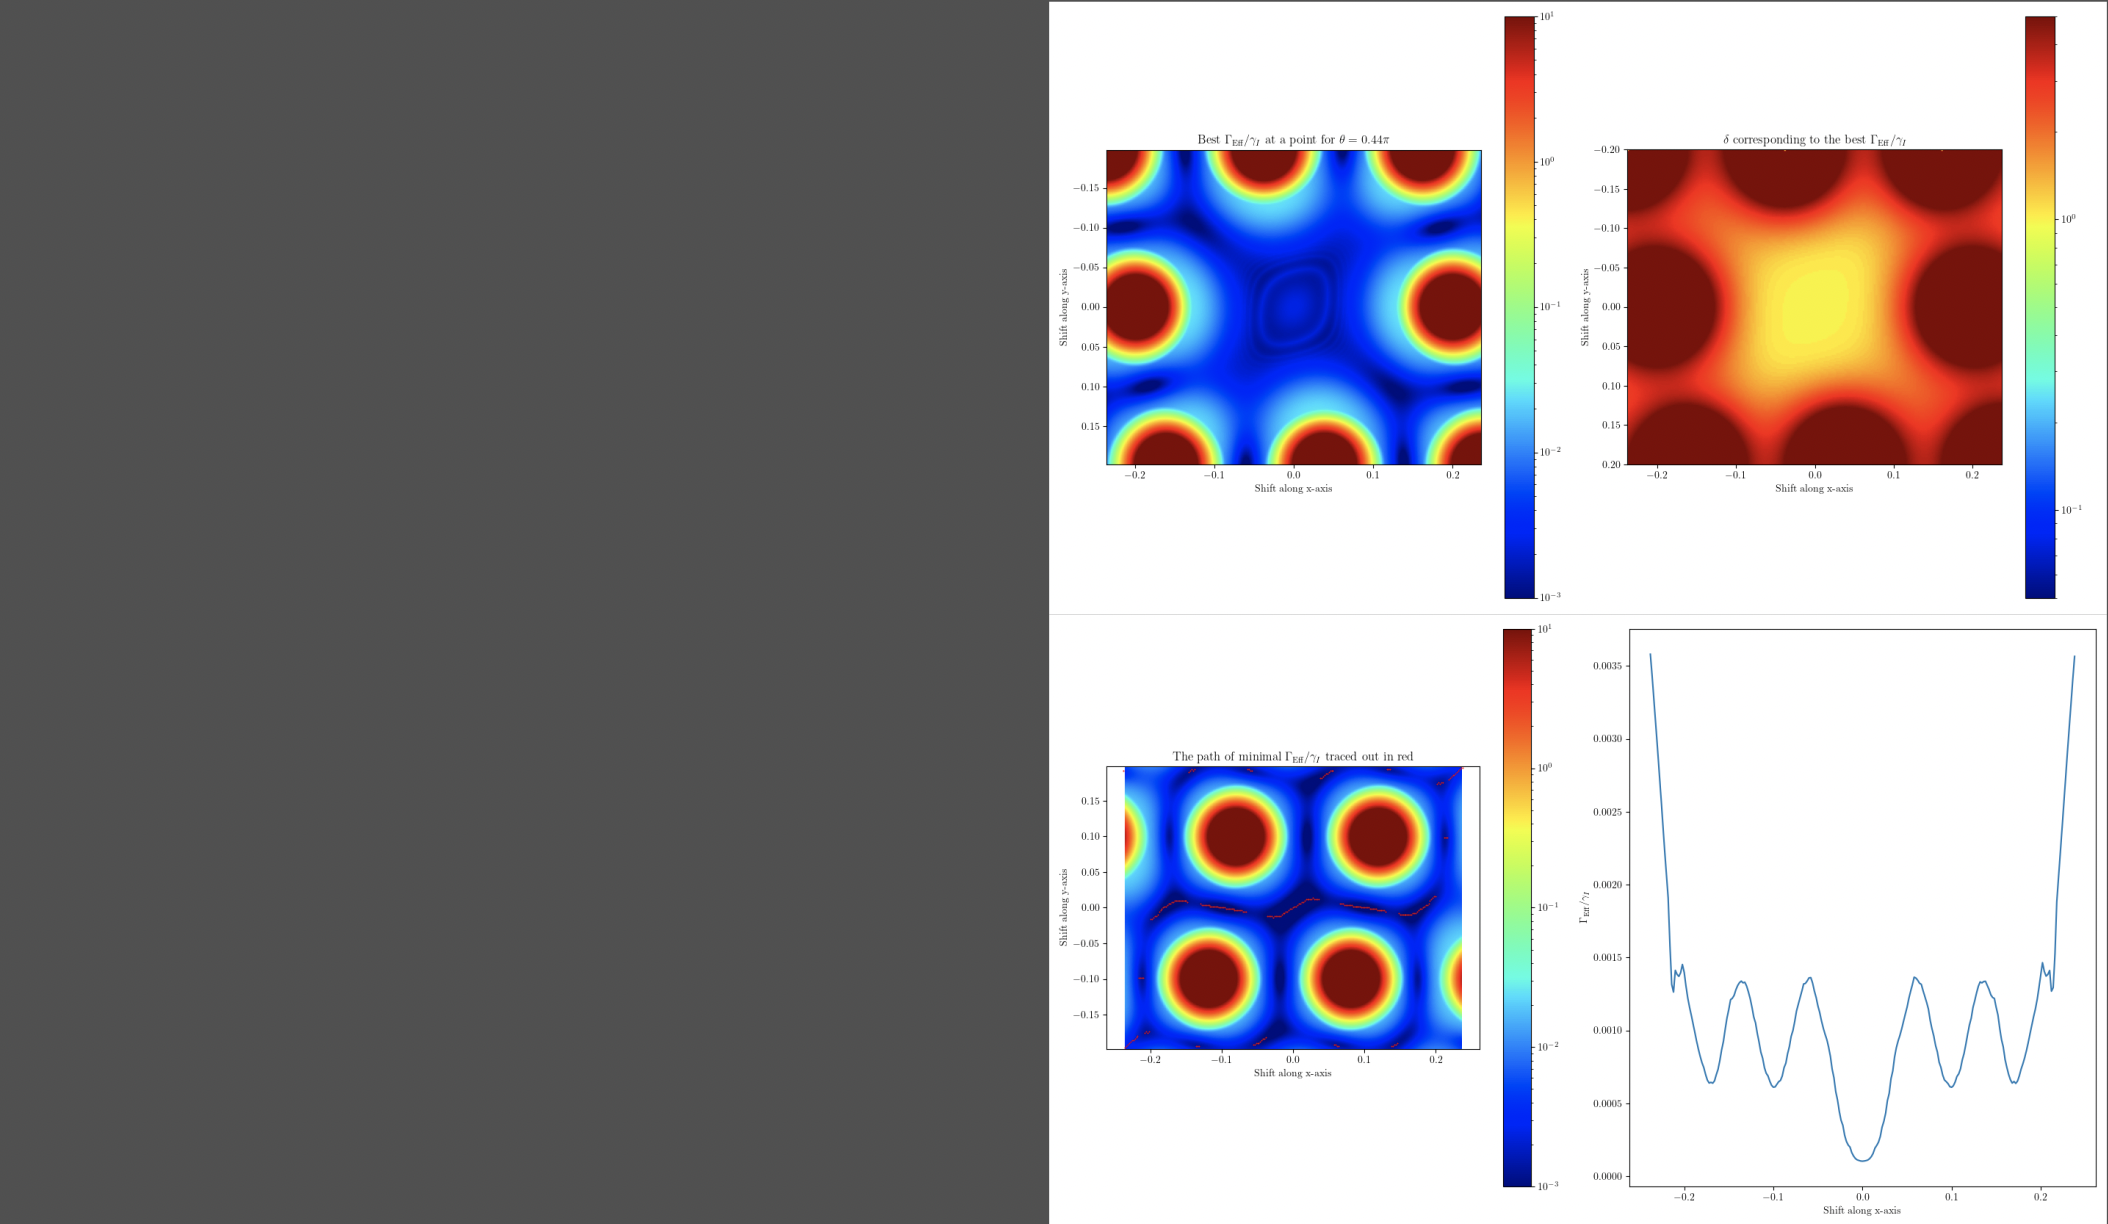
\includegraphics[width=1.0\textwidth]{figures/mono_rect_plaquettes_interstitial.png} 
    \caption{•}
    \label{fig:mono_rect_plaquette_interstitial}
\end{figure*}


%=================
\subsubsection{Substitution}

\begin{figure*}
    \centering
    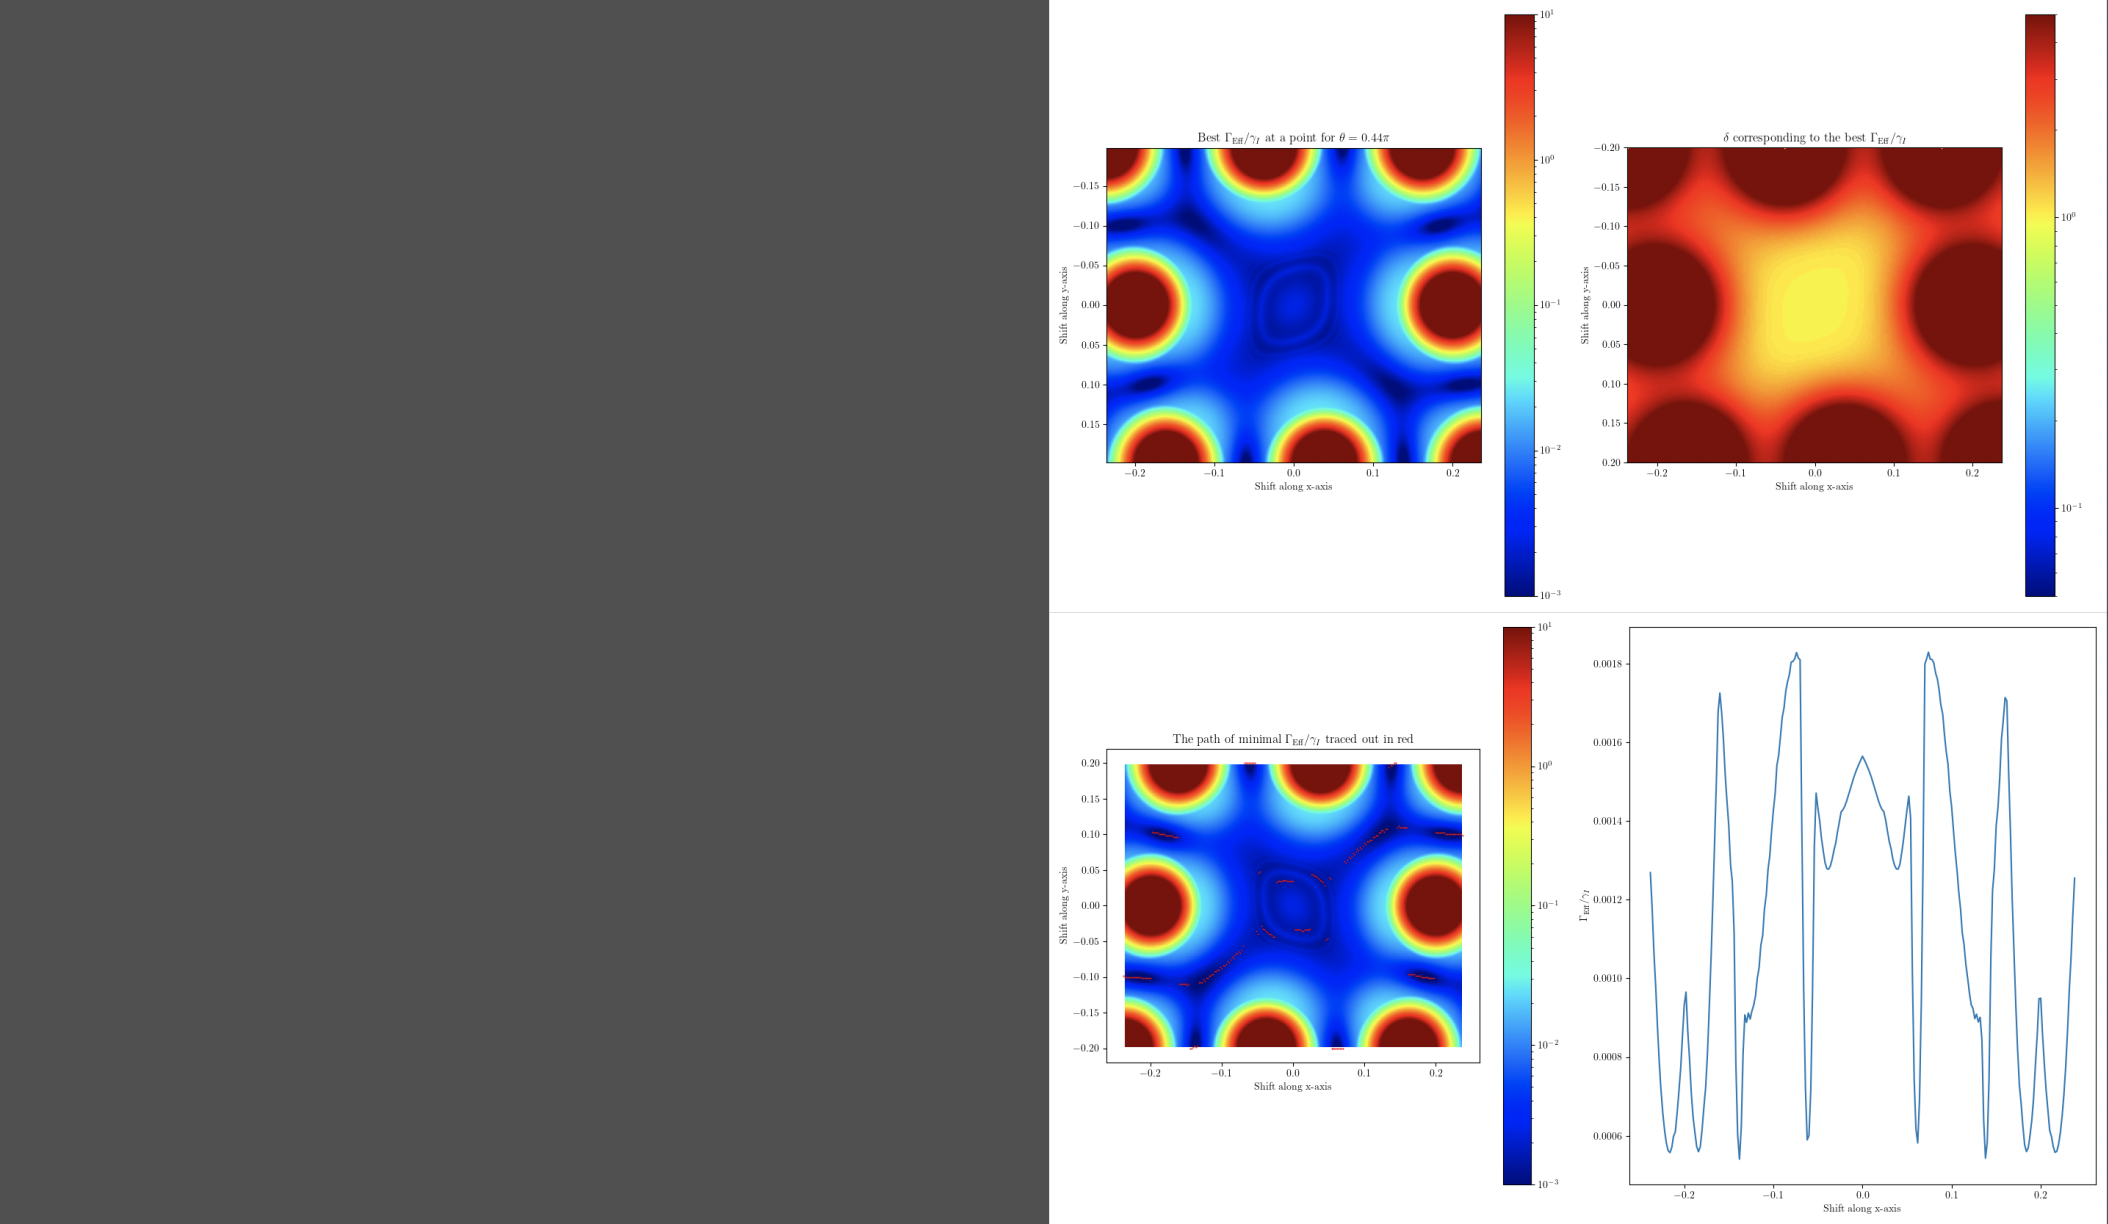
\includegraphics[width=0.4\textwidth]{figures/mono_rect_plaquettes_substitution.png} 
    \caption{•}
    \label{fig:mono_rect_plaquette_substitution}
\end{figure*}

%=================
\subsubsection{Varying scaling factors}
\commentSO{justify why we use interstitial in the following}

\begin{figure}
    \centering
    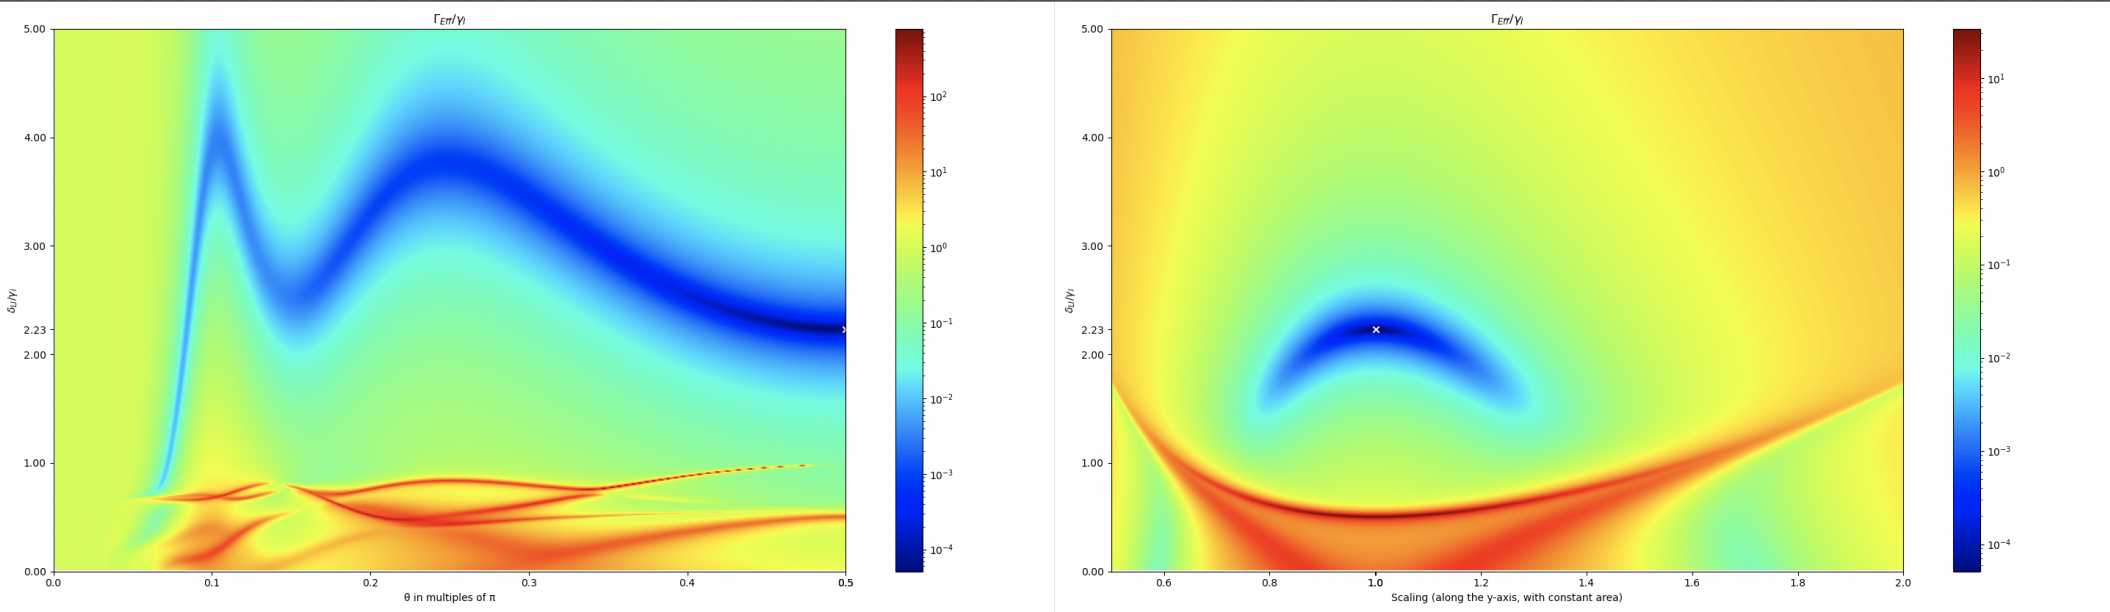
\includegraphics[width=0.4\textwidth]{figures/mono_rect_thetadelta.png} 
    \caption{•}
    \label{fig:mono_rect_thetadelta}
\end{figure}


%==============================================================================================
\section{Two impurity case}
\commentSO{Q-factor, analyze different lattices -> discuss the most important figures, constant distance}

$\Gamma_\text{eff}$ for a lattice with two impurities is calculated in a manner analagous to the single-impurity case, starting with the Schr\"odinger equation for the two-impurity Hamiltonian, for which 

% \commentSB{Perhaps write out the meanings of all these new variables, if it's not clear}
\begin{equation}
    i \hbar \begin{pmatrix}
        0 \\ \vdots \\ 0 \\ \dot{c} \\ \dot{d}
    \end{pmatrix}
    = \begin{pmatrix}
        ~ & ~ & ~ &   C_{L1} & C_{L2} \\ 
        ~ & H_L & ~ & \vdots & \vdots \\
        ~ & ~ & ~ & C_{L1} &  C_{L2} \\
        C_{1L} & \cdots & C_{1L} & H_1 & C_{12} \\
        C_{2L} & \cdots & C_{2L} & C_{21} & H_2  
    \end{pmatrix} 
    \begin{pmatrix}
        b_1 \\ \vdots \\ b_N \\ c \\ d
    \end{pmatrix}
    \label{eqn:blockH2}
\end{equation} 
In this way, 
\begin{equation}
    b = -(H_L)^{-1} (C_{L1} c + C_{L2} d)
\end{equation}
Putting this result back into the Schr\"odinger equation gives
\begin{subequations}
\begin{align}
    \dot{c} &= -i \left[  H_1 - {C_{1L}}^T (H_L)^{-1} C_{L1}\right] c \nonumber\\
     &\quad- i \left[  C_{12} - {C_{1L}}^T (H_L)^{-1} C_{L2} \right]  \\
    \dot{d} &= -i \left[  H_2 - {C_{2L}}^T (H_L)^{-1} C_{L2}\right] c \nonumber\\
     &\quad- i \left[  C_{21} - {C_{2L}}^T (H_L)^{-1} C_{L1} \right] d 
\end{align}
\end{subequations}
Let $\dot{c} = -i [\Sigma_1 - \frac{i \gamma_1}{2}]c - i \kappa_1 d $ and $\dot{d} = -i [ \Sigma_2 - \frac{i \gamma_2}{2} ] d - i \kappa_2 c $, where $\kappa_1$ and $\kappa_2$ are ``effective couplings.'' Solving for these and the self-energies results in 
\begin{subequations}
    \begin{align}
        \Sigma_1 = H_1 - {C_{1L}}^T (H_L)^{-1} C_{L1} + \frac{i \gamma_1}{2} \\
        \Sigma_2 = H_2 - {C_{2L}}^T (H_L)^{-1} C_{L2} + \frac{i \gamma_2}{2} \\
        \kappa_1 = C_{12} - {C_{1L}}^T (H_L)^{-1} C_{L2} \\
        \kappa_2 = C_{21} - {C_{2L}}^T (H_L)^{-1} C_{L1} 
    \end{align}
\end{subequations}

The impurities' effective decay rates are determined by $\Gamma_\text{eff,i} = \gamma_1 - 2~\im[\Sigma_i]$, where $i$ stands for either the first or second impurity. Likewise, we define the Q-factor as a function of the effective decay rate and the effective coupling, so that $ Q_i = \frac{\re[\kappa_i]}{\Gamma_\text{eff,i}} $ for each of the two impurities. Because the first and second impurities occupy symmetric positions in the lattice, we find that $\Gamma_\text{eff,1} = \Gamma_\text{eff,2}$ and $Q_1 = Q_2$. We thus consolidate these variables, so that we may speak of the impurities' effective decay rate $\Gamma_\text{eff}$ and overall quality factor $Q$. 

% \commentTP{Put these in-line, and consolidate them into single equations of the form $\Gamma_\text{eff:1,2}$. And mention that the 1 and 2 equations are equal to each other because we choose that to be the case, and so we can really just atlk about a single Geff and a single Q}



%=================
\subsection{Monoclinic lattice}


%=================
\subsection{Rectangular lattice}


%==============================================================================================
\section{Conclusions and Outlook}\label{sec:conclusion}

These are the Conclusions.\\[2ex]

\emph{Acknowledgments.} We would like to thank \commentSO{add people}. This work was supported by \commentSO{add funding sources}

The numerical simulations were performed with the open-source framework \texttt{QuantumOptics.jl}~\cite{kramer_quantumopticsjl_2018}.


\bibliographystyle{apsrev4-1-title}
\bibliography{references_optimized_geometries}

\end{document}

